% !TEX TS-program = pdflatex
% !TEX encoding = UTF-8 Unicode

% This is a simple template for a LaTeX document using the "article" class.
% See "book", "report", "letter" for other types of document.

\documentclass[a4paper, 12pt, english]{scrreprt} % use larger type; default would be 10pt
% \documentclass[bibliography=totocnumbered, 12pt]{report}

% \usepackage[utf8]{inputenc} % set input encoding (not needed with XeLaTeX)

%%% Examples of Article customizations
% These packages are optional, depending whether you want the features they provide.
% See the LaTeX Companion or other references for full information.

%%% PAGE DIMENSIONS
\usepackage[inner=2.5cm, outer=2.5cm, bottom=4cm, top=3cm]{geometry} % to change the page dimensions
% \geometry{a4paper} % or letterpaper (US) or a5paper or....
% \geometry{margin=2.5cm} % for example, change the margins to 2 inches all round
% \geometry{landscape} % set up the page for landscape
%   read geometry.pdf for detailed page layout information

\usepackage{graphicx} % support the \includegraphics command and options
\usepackage[font=footnotesize]{caption}

% \usepackage[parfill]{parskip} % Activate to begin paragraphs with an empty line rather than an indent

%%% PACKAGES
\usepackage{booktabs} % for much better looking tables
\usepackage{array} % for better arrays (eg matrices) in maths
\usepackage{paralist} % very flexible & customisable lists (eg. enumerate/itemize, etc.)
\usepackage{verbatim} % adds environment for commenting out blocks of text & for better verbatim
\usepackage{subfig} % make it possible to include more than one captioned figure/table in a single float
\usepackage[sorting = none]{biblatex}
% \usepackage{biblatex}
\usepackage{url}
% These packages are all incorporated in the memoir class to one degree or another...

%%% HEADERS & FOOTERS
\usepackage{fancyhdr} % This should be set AFTER setting up the page geometry
% \pagestyle{fancy} % options: empty , plain , fancy
\renewcommand{\headrulewidth}{0pt} % customise the layout...
\lhead{}\chead{}\rhead{}
\lfoot{}\cfoot{\thepage}\rfoot{}

%%% SECTION TITLE APPEARANCE
% \usepackage{sectsty}
% \allsectionsfont{\sffamily\mdseries\upshape} % (See the fntguide.pdf for font help)
% (This matches ConTeXt defaults)

\usepackage{mathtools}
\usepackage{hyperref}
\usepackage{longtable}
\usepackage{booktabs}
\usepackage{float}
\usepackage{amsfonts}
\usepackage{lscape}

% \usepackage[nottoc,notlot,notlof]{tocbibind} % Put the bibliography in the ToC
% \usepackage[titles,subfigure]{tocloft} % Alter the style of the Table of Contents
% \renewcommand{\cftsecfont}{\rmfamily\mdseries\upshape}
% \renewcommand{\cftsecpagefont}{\rmfamily\mdseries\upshape} % No bold!

% \usepackage{fontspec}
% \setmainfont{Arial}
\usepackage{setspace}


\usepackage{algorithm}
\usepackage{algpseudocode}
% \usepackage[toc, title, page]{appendix} 

\bibliography{bibliography}


\title{TESI}
\author{Claudia Sessa}
% \date{} % Activate to display a given date or no date (if empty),
         % otherwise the current date is printed 

\begin{document}
% \maketitle

%\section{First section}
%
%Your text goes here.\\
%Mamao mamao bacini tanti tanti
%ihihih
%
%\break
\singlespacing
\tableofcontents

\doublespacing
\chapter{Introduction} \label{ch:intro}


Transportation systems are very complex, as they involve many components and stakeholders. Among the main challenges of recent years there is that of creating a mobility infrastructure that satisfies the needs of all stakeholders, in terms of efficient movement, sustainability, safety and accessibility. The increase in population in urban centers has made it more challenging for transportation companies and public authorities to maintain high quality standards of the transportation services. In this context, transport models, digital replicas of these complex real-world systems, can be seen as a powerful tool for assessing the efficiency of transport infrastructures, and for predicting future performance in response to the dynamic needs of users. Transport models allow planners to understand the current issues in their transportation system, to identify opportunities, and to design reliable and resilient services which optimally serve passengers needs. 
In this regard, the city of Milan provides an interesting case study, with its transportation system including a total of 143 routes among metro, tram, bus and filobus, managed by Azienda Trasporti Milanesi (ATM), as well as taxi, car, bike and scooter sharing services. Every year, ATM services host around 585 million passengers, spending, on average, 43 min on public transport per day \cite{bib2}. The goal of this research is to propose a model for the demand on Milan's public transportation system, which can be used to project future demands, to test in advance the impact of interventions and changes to the network, as well as the application of polices in the mobility sector. In other words, the proposed model is a tool that attempts to evaluate the network efficiency from the emergence of issues, which in practice arise daily, such as long waiting times at the stops, overcrowded vehicles and sudden changes of the network. For simplicity, I only focus on the public transportation system and on the share of daily passengers relying on the public service.
This research is articulated around two main questions:
\begin{enumerate}
    \item Is it possible to construct a model that reproduces Milan's transportation system's infrastructure and simulates the flows of passengers making use of the service, in a way that allows evaluating how much the system is efficient in meeting users' demand?
    \item Given that it is possible to construct such a parametric model for public transportation, which are the elements to which the model is more sensible? How do model results vary in response to changes in parameter values?  
\end{enumerate}
I will show that a suitable framework to achieve the first goal of the analysis is that of Agent-based Modeling (ABM), a flexible simulation technique allowing to model a system from its constituent units. Since the information about individual trips is restricted, as Origin-destination (OD) matrices\footnote{Origin Destination Matrix contains the starting point and end point of individual trips, and it could be obtained through surveys or directly from devices owned by the transportation company, as in the ATM case. It provides a description of movements in a certain geographic area, and is used to assess the demand for transportation.} are owned by ATM, I needed to come up with a way to replicate the passenger flow. I will describe a synthesis procedure, based on publicly available aggregate statistics about the population, which will be used to create the synthetic agents to be fed to the model and simulate passengers and their travel behavior. Later, I will address the second question through a Sensitivity Analysis of the model, with respect to its parameters and "non-parametric" elements, a procedure which allows gathering insights about the dependencies and validity of the ABM's results. \\ 
Specifically, in Chapter \ref{ch:literature}, I will present an overview of the two theoretical frameworks at the basis of this research, Agent-based Modeling and Sensitivity Analysis, as to provide the readers with the concepts that are relevant for the following chapters. \\ Then, Chapter \ref{ch:model} is dedicated to a detailed explanation of the model for passengers' flow on Milan's public transportation network. Finally, in Chapter \ref{ch:sa} I will carry on a local Sensitivity Analysis of the model, following the protocol that has been recently proposed by \textcite{Borgonovo2022SensitivityAO}.

Both the simulator and the Sensitivity Analysis have been developed in Python 3.9, and the main libraries exploited are Pandas \cite{mckinney-proc-scipy-2010} and NetworkX \cite{SciPyProceedings_11}. The data and the code are available at [METTERE LINK GITHUB].
\chapter{Agent-based Modeling and Sensitivity Analysis} \label{ch:literature}

The purpose of this chapter is to briefly introduce the reader to the two main theoretical frameworks of this thesis: Agent-Based Modeling (ABM) and Sensitivity Analysis. In particular, in Sections \ref{abm} and \ref{abm-t} I present the ABM framework: first, I provide a general overview of Agent-based Modeling; then, I focus on how this modeling technique is applied in the field of transportation, the most related to this thesis. In Section \ref{sec:ch2_sa} I introduce the topic of Sensitivity Analysis, and describe the goals one can achieve through it. Finally, in Section \ref{sa-abm}, I present the main techniques to perform sensitivity analysis of agent-based Models.  

%%%%%%%%%%%%%%%%%%%%%%%%%%%%%%%%%%%%%%%%%%%%%%%%%%%%%%%%%%%%%%%%%%%%

\section{Agent-based Modeling}\label{abm}

Agent-based modeling (ABM) is a simulation technique that allows to describe complex systems with a "bottom-up" approach, meaning by specifying the behavior of the smallest components of the system and then connecting them to be able to generate simulated data about the system functioning that can be analyzed inductively. \textcite{bonabeau2002} defines agent-based models as \textit{"a mindset more than a technology"}, highlighting that one can think of ABM as \textit{microscopic modeling}, as opposed to \textit{macroscopic modeling}, in which one needs to specify the theory and, hence, the equations ruling the system. Indeed, agent-based models are particularly suitable when a high number of equations are required in order to fully specify the system, and the typical "top-down" approach used in equation-based models (EBMs) becomes unfeasible (figure \ref{abm_bu}). Indeed, as suggested by \textcite{Walton2007ArtificialII}, \textit{"a traditional model develops equations to describe the observed characteristics, while an ABM uses rules or equations to describe the individual behaviors"}. \\

\begin{figure}
    \centering
    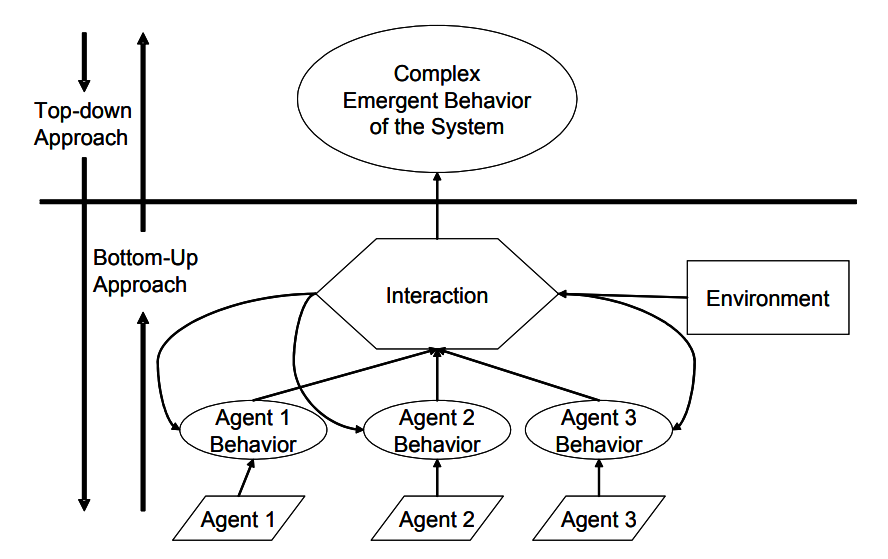
\includegraphics[width=0.8\textwidth]{tex/pics/abm_bottomup.png}
    \caption{Two approaches to model a complex system. Adapted from \textcite{bernhardt2007agent}.}
    \label{abm_bu}
\end{figure}

In general, an ABM is defined by four main elements:
\begin{itemize}
    \item \textbf{The agents}, or computational individuals;
    \item \textbf{The environment}, in which agents are located and move;
    \item \textbf{The time}, and, in particular, the unit of time;
    \item \textbf{The rules}, determining the behaviour of the agents, their interaction and evolution.
\end{itemize}
In agent-based models, a system is described as a collection of autonomous, identifiable entities, called agents, who take decisions and interact between themselves and with the environment in which they are located. Modeling these interactions allows us to capture dynamics and emergent phenomena which otherwise would be unpredictable and impossible to analyze. The interactions are determined both by the rules of the model and by the topology of the environment, which dictates who gets in contact with whom. In fact, just as in real-world, not all agents interact directly with all the other agents all the time, but only with a subset of other agents constituting their \textit{neighborhood}. Typical topologies for ABMs' environment (figure \ref{topologies}) are the "Cellula Automata" (endowed with either von Neumann ‘4-neighbour’ neighbourhood or Moore's ‘8-neighbour’ neighbourhood), Euclidean spaces, Network structures, the Geographic Information System (GIS) topology, and the 'soup' (where agents' location is irrelevant).  \\

\begin{figure}
    \centering
    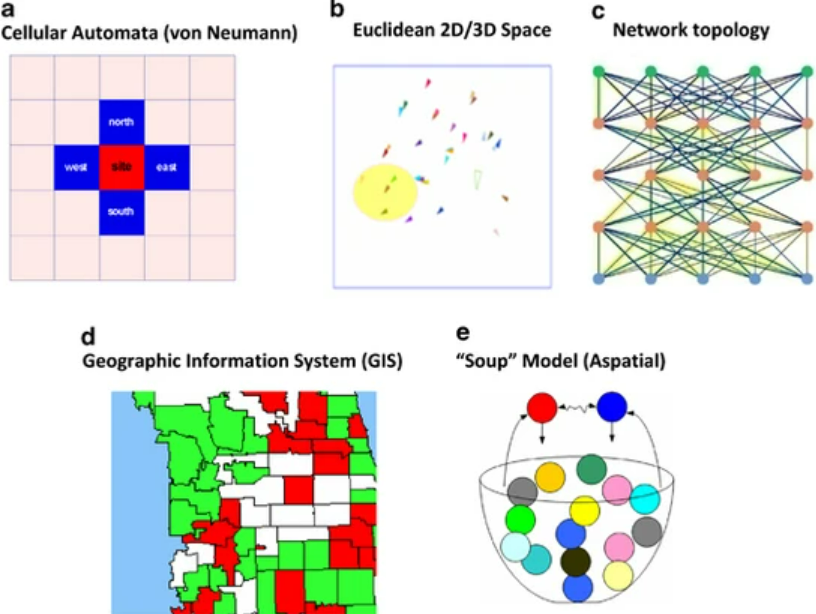
\includegraphics[width=0.7\textwidth]{tex/pics/abm_topologies.png}
    \caption{Common topology structures for ABMs environment. Adapted from \textcite{tutorialABM1}.}
    \label{topologies}
\end{figure}

Agents are characterized by attributes, describing their profile and making them identifiable, and by a state, which varies over time. Attributes allow to potentially define each agent as a different individual exhibiting a different behavior, as to account for real-world heterogeneity. Depending on their state, agents have different admissible actions, which determine their possible behavioral patterns. The individual decision-making process can be modeled with simple, deterministic \textit{if-then} conditional rules, but also with complex probabilistic or mixed rules. Neural networks and genetic algorithms may also be employed, as in \textcite{ALKINANI20228325, abm_rl}, to make the decision-making process more sophisticated and flexible. Usually, agents are "goal-directed", having goals to achieve and/or objective functions to optimize, and adapting their behavior at next steps on the outcome of previous iterations. Indeed, such kind of model is preferred when it is crucial to have agents that learn and adapt their behavior over time.
Object-oriented programming (OOP) languages are a natural choice to construct agent-based models. Indeed, both agents and environment can be implemented as objects, with their attributes and methods representing the rules of the model. \\
  
Agent-based models have recently become increasingly popular, due to their numerous advantages, among which the following should be mentioned:
\begin{itemize}
    \item \textbf{The flexibility}, or the ability to change the degree of description of agents and rules. In particular, one may want to run the simulation with all the agents or a subgroup of agents, or to evolve agents' attributes and rules at any time. This allows to obtain a model with a high level of realism. 
    \item \textbf{The bottom-up approach}, allowing to model the heterogeneity of agents and to describe the system in a more natural way than by specifying a set of equations.
    \item \textbf{Ability to capture emergent phenomena}, arising from the interactions of the individuals under the specified rules, when their collective behavior is much more complex than the sum of each individual behavior. 
\end{itemize}
Although in many fields ABM appear to be the most natural way to represent a system, some weaknesses of this modeling technique should be mentioned. First, ABMs typically require huge amounts of data to be validated, and such data are not always available, especially in the case of systems which have not been extensively studied yet. Moreover, as suggested by \textcite{parunak}, \textit{"the code needed to represent an agent’s behavior in ABM is often longer and more complex than a typical equation in an EBM, and thus potentially more susceptible to representational error"}, which is the error deriving from an inexact representation of the system under study. One last practical issue is that the execution of ABMs simulations can be computationally intensive and time-consuming, an issue that can be at least partly overcome by employing adequate hardware resources and optimizing the code. \\

Despite the aforementioned drawbacks, agent-based models have proved to be a versatile technique. The earliest ABM application is thought to be Shelling's model for racial segregation from 1971 \cite{shelling71}, which he used to demonstrate the spontaneous development of ghettos in social systems. Lately, models of this type have been used in many disciplines, such as physics, biology, but also management sciences, social sciences, economics and ecology. Applications range from models for the immune system \cite{Folcik2007TheBI} to models for existing or hypothetical markets \cite{Charania2006SubOrbitalST, markets2, market3} and for organizational behavior \cite{organization}. Recent applications include models for epidemics and, in particular, COVID-19 pandemic spread \cite{covid1, covid2, covid3}. In the next Section, I will focus on applications in the transportation field, which is the main interest of this thesis.


%%%%%%%%%%%%%%%%%%%%%%%%%%%%%%%%%%%%%%%%%%%%%%%%%%%%%%%%%%%%%%%%%%%%%%%

\section{ABM in the transportation field} \label{abm-t}
In the transportation field, agent-based modeling is particularly appropriate to model such systems in which human actions play a critical role. When searching for literature about agent-based models in transportation, a first categorization of the results appears to be evident. There are two main categories in which results can be classified: models for transportation in the context of supply chain and logistics, and models for urban mobility. The two have many points in common, as they both typically imply some vehicle usage and the need to optimize the route such vehicles have to travel, and they often focus on critical situations, like traffic congestion. In general, however, they have different scopes and involve different categories of agents. 

ABMs for logistics attempt to describe the process of freight transport and distribution, which can produce significant economic, social and environmental impacts. In these models, the agents are the main actors in the supply chain that make logistic decisions. In particular, agent based freight models like \cite{log1, log2} identify three main categories of agents: the suppliers (goods' producers, wholesalers and shippers who supply the goods), the receivers (retailers and end-consumers), and the transport providers (freight carriers, couriers or third party logistic service providers taking care of transportation). Some papers use ABMs to control the effects of measures and policies in the transportation sector \cite{log3, log4}; others, instead, aim at solving vehicle routing problems given dynamic decision-making strategies, taking into account external factors, such as road traffic and freight demand \cite{log5}. 

On the other hand, ABMs for urban mobility are used to schematize citizen's behaviour in order to observe population-level dynamics.
\textcite{bernhardt2007agent} identifies four problems related to transportation, and, in particular, related to urban mobility, for which there is an extensive ABM literature: traffic simulation\footnote{There exist several ABM-based simulators for traffic simulation, of which two of the more widely known are TRANSIMS (\url{http://transims.tsasa.lanl.gov/}) and MATSIM (\url{http://www.matsim.org/}).}, pedestrian simulation, lane-changing and travel-demand modeling.  
Agents of ABMs for urban mobility represent the individuals living in and moving around the city, with methods to decide the route to follow and to enable interactions. The real population of the city is often represented, as accurately as possible, by generating a synthetic population, calibrated on socio-demographic information from census data \cite{bib6}. Each agent’s behaviour and movements can be determined through the assignment of a travel diary \cite{bib7}, a sequence of activities the individual makes in a representative work day, with details such as departure time, origin and destination. This approach is called “activity-based” \cite{bib8} or “activity-based travel demand model” \cite{bib3} and it has been adopted in several works to study mobility systems of different cities. Its main characteristic is that travel decisions are driven by a collection of activities that form an agenda. The activities are scheduled along with the time, location and means of transport used.
In some cases, also vehicles are modeled as agents of the model, with methods allowing them to move on the network, embark and disembark people. \textcite{Bazghandi_techniques} adds also routes, intersections and signals as possible agents of the model. \\

% LITERATURE OF MODELS SIMILAR TO MINE
The focus of this research is on this second category of models (ABMs for urban mobility) and in particular on cities' public transportation network, to evaluate the efficiency of the public service and the effects of interventions. The idea of using an ABM to study individuals’ mobility patterns is not new in the field of urban science. In \textcite{bib9}, the authors have built an ABM to study the impact of different mobility modes on traffic flow and congestion, with a focus on the city of Cambridge. Another related work is \textcite{bib7}, in which authors have simulated land use and transport demand of an urban area of Sydney. As for Milan, several analyses have been conducted concerning the integration of shared mobility services into the public transport network, the latest ones focusing on how to respond to new needs generated by the pandemic, as in \textcite{bib10}. Still with respect to the pandemic, in \textcite{bib11} adopted a simulation approach to evaluate different unlock strategies for public transportation. No significant work has been published yet which considers the flow of passengers as a determinant of the efficiency of Milan’s transport network. The proposed model, presented in details in Chapter \ref{ch:model}, aims at closing this literature gap. 


%%%%%%%%%%%%%%%%%%%%%%%%%%%%%%%%%%%%%%%%%%%%%%%%%%%%%%%%%%%%%%%%%%%

\section{Sensitivity Analysis} \label{sec:ch2_sa}

% 1. What is SA
%   1.1 Definition and why it is useful
%   1.2 Difference from MV and UA
Sensitivity Analysis (SA) is \textit{"the study of how the uncertainty in the output of a model  (numerical or otherwise)  can  be  apportioned to  different  sources  of uncertainty in the model input"} \cite{Saltelli2002SensitivityAF}. 
Given a decision-support model (or, in short, model), \textcite{RAZAVI2021104954} identify several purposes a researcher can address through sensitivity analysis:
\begin{itemize}
    \item Scientific discovery, to explore how the combinations and interactions of hypotheses and parameters affect the system simulated through the model;
    \item Dimensionality reduction, to reduce the complexity of the model;
    \item Data worth assessment, to identify the factors for which one would want to acquire more data;
    \item Decision support, to quantify the sensitivity of an expected outcome to assumptions and constraints.
\end{itemize}

SA differs from Model Validation, which, consists in collecting data both for the input and the output and checking how well the model fits reality. However, according to \textcite{Gass1983FeatureA}, SA is an element of Operational Validity, which is concerned with ensuring a model is able to produce the expected answers given the inputs, allowing the decision maker to accept or reject it.
Sensitivity Analysis also differs from Uncertainty Analysis (UA) (figure \ref{fig:sensitivity_saltelli}), which ideally should be performed before it, and consists in quantifying the uncertainty in the outputs of the model without attempting to attribute it to any particular input. SA, instead, allows us to decompose the uncertainty that propagates through the model into its sources.

\begin{figure}[H]
    \centering
    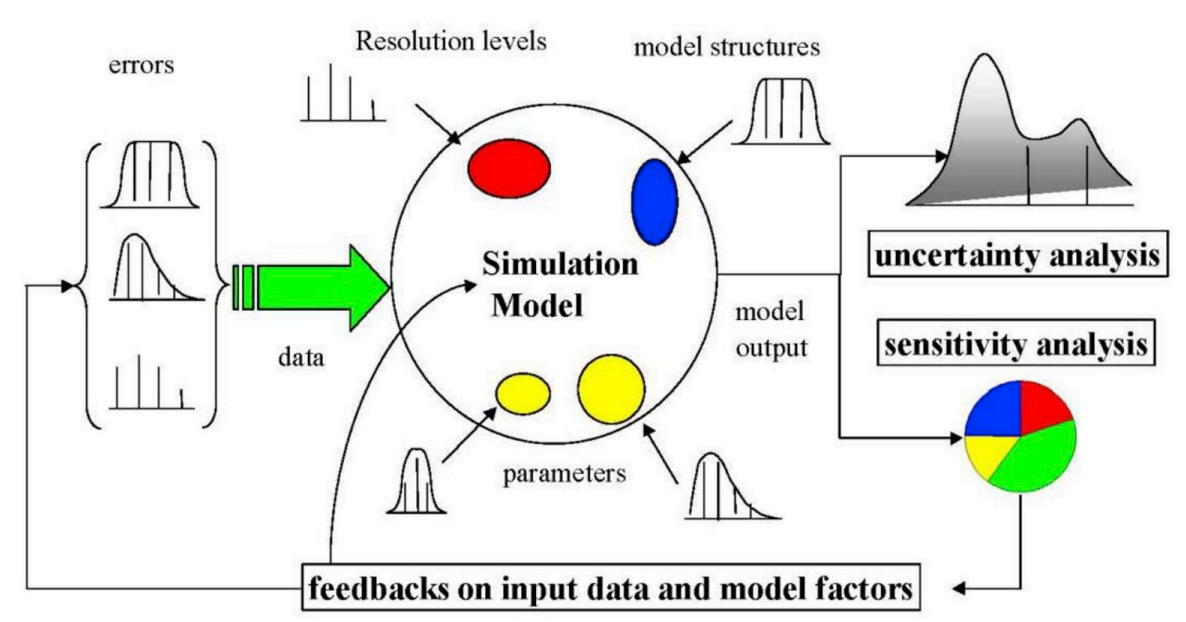
\includegraphics[scale = 0.7]{tex/pics/sensitivity_saltelli.png}
    \caption{Uncertainty and Sensitivity Analysis of a decision model. The grey curve represents the empirical distribution of the output of interest, given that uncertainty propagated from inputs through the model. The pie chart shows the decomposition of uncertainty into its different sources. Adapted from \textcite{saltelli}.}
    \label{fig:sensitivity_saltelli}
\end{figure}

%   1.3 Terminology (model/input/output)
%   1.4 Deterministic vs Stochastic model
When performing Sensitivity Analysis, the decision model is regarded as a map \textit{g} from the input space \textit{X} to the output space \textit{Y}: $g: \mathcal{X} \rightarrow \mathcal{Y}$. Given n model inputs and D outputs, then one can define $X \subseteq \mathbb{R}^n$ and $Y \subseteq \mathbb{R}^D$. Let the vector of model inputs be $\mathbf{x} = (x_1, x_2, ..., x_n)$. It may be the case that not all inputs are the subjects of the sensitivity analysis, so one can construct the index set of inputs which are taken into consideration $\alpha = (i_1, ..., i_k)$ where $k\leq n$ and the corresponding input vector would be $\textbf{x}_{\alpha} = (x_{i_1}, x_{i_2}, ..., x_{i_k})$. In this setting, one can formalize the difference between a deterministic and a stochastic model. Indeed, a model is said to be deterministic, if by fixing its input \textbf{x} to a value $\textbf{x}^0$, the output remains unchanged \cite{Borgonovo2017SensitivityAA}. Conversely, if a model produces a random value any time it is run with the same fixed input $\textbf{x}^0$, then it is said to be stochastic. In this case, the analyst would be interested in the conditional distribution of the output given that the input is fixed at $\textbf{x}^0$. Formally speaking, a deterministic model is a particular case of a stochastic model, where the output is a Dirac-$\delta$ function centered at $\textbf{x}_0$. If the model is deterministic, then running the model repeatedly with different inputs and propagating the uncertainty from inputs to outputs is enough to assess the uncertainty in the outputs. 

% 2. The Sensitivity question + SA Settings 
% 3. Deterministic vs Probabilistic frameworks/methods for sensitivity
Before performing sensitivity analysis, a crucial step is to state the goal of the analysis, meaning the insights one is looking for. Formulating the wrong sensitivity question may lead to the use of unsuitable methods and, hence, to obtain wrong or useless insights from the analysis. A first consideration to be made is whether one wants to perform a Local or Global sensitivity analysis. In local sensitivity analysis, one varies the input around a reference value, making finite perturbation. This happens in a deterministic framework, as no probability distribution is assigned to the input. In global sensitivity analysis, instead, the researcher spans the entire input space to assess how interactions of the inputs on the full problem space affect the outputs of the model. If a probability distribution for the inputs is specified, one speaks of probabilistic sensitivity analysis. In this setting, the input vector is a random vector $\textbf{X} = (X_1, ..., X_n)$, whose realizations are $\textbf{x} = (x_1, ..., x_n)$, with cumulative distribution $F_{\textbf{X}}(\textbf{x})$. Uncertainty in the model inputs makes the output y a random variable Y = g(X), of which one could compute statistics. In practice, the modeler runs simulations by generating samples of the inputs, evaluating the model for each sample as to obtain samples of the model outputs through which are obtained the empirical cumulative distribution functions of the outputs.

To formalize the choice of the sensitivity question, researchers have developed the concept of sensitivity analysis settings \cite{Saltelli2002SensitivityAF, Saltelli2002OnTR}, representing goals of sensitivity analysis, but also the main corresponding methods used to achieve them. \textcite{Borgonovo2016SensitivityAA}, in their literature review, define a setting as \textit{"a formulation of the sensitivity analysis quest which is stated before the sensitivity analysis is carried out"}, and identify five main settings:
\begin{itemize} \label{sa_settings}
    \item \textbf{Factor prioritization}: the goal is to identify the main drivers of output changes, according to some importance measure, to be able to focus resources in data collection on the acquisition of data related to the most important inputs as to reduce uncertainty in the results. Appropriate methods are finite differences (with total effects visualized through Tornado diagrams), in deterministic frameworks, or differentiation-based measures, in probabilistic analysis.
    \item \textbf{Factor fixing}: here the goal is similar but opposite to that of factor prioritization: identifying the least influential parameters, which can then be fixed as to reduce complexity of the model and save computational cost.
    \item \textbf{Direction of change}: in this case, one is interested to know whether an increase (or a decrease) in a model input provokes an increase (or a decrease) in model outputs. For example, one may want to look at the sign of finite change sensitivity indices or of partial derivatives, in the deterministic and probabilistic framework respectively.
    \item \textbf{Interaction quantification}: the goal is to analyze the structure of the model to understand whether there are interactions among the model inputs. Usually, researchers focus on two-elements interactions, since higher-level interactions are computationally expensive to analyze.
    \item \textbf{Robustness (or Stability)}: decision-makers are interested in determining whether variation to parameters' reference value invalidate the conclusions of the analysis and assessing the region of the model input space over which, instead, there is no change.
\end{itemize}



%%%%%%%%%%%%%%%%%%%%%%%%%%%%%%%%%%%%%%%%%%%%%%%%%%%%%%%%%%%%%%%%%%

\section{Sensitivity Analysis of ABMs} \label{sa-abm}


% 1. perchè fare sa degli abm
% 2. challenges?
%     - two levels (micro vs macro)
%     - stochastic --> min simulation runs
%     - spatio-temporal outcome
% 3. methods
% 4. borgo steps

In order for an ABM to be useful to learn about a complex system, it is essential to compare the effects on output measures under different parameters configurations. Sensitivity analysis allows examining the robustness of the model to parameter changes, to ensure that the conclusions one takes do not depend on specific sets of assumptions. Analyzing the behavior of the model becomes even more crucial if the researcher is interested in capturing, through the model, early signals of the system being in a critical condition. Indeed, SA helps to identify the hidden model dynamics, by inspecting the effects of parameter changes into model output. Moreover, it plays an important role in recognizing if there are computationally expensive assumptions of the model that can be replaced with cheaper ones without compromising the results.  

There are, however, several structural properties of ABMs that make the application of statistical methods to perform sensitivity or uncertainty analysis quite challenging in this framework. First, agent-based models have at least two levels of detail: a \textit{micro-level}, consisting of everything concerning agents and their individual behavior, and a \textit{macro-level}, comprising the environment and the emerging macroscopic patterns. This duality is also reflected in the results of ABM simulations, as one typically obtains both individual-level and system-level outputs, gaining distinct managerial insights. Moreover, interactions between agents are typically non-linear and may change over time, due to agents' learning and emergent dynamics. With non-linear individual interactions, there might be also non-linear input-output relations, which may be difficult to capture adopting standard sensitivity methods. As a consequence, similar parameters may lead to totally different outputs, while completely different settings could produce similar system behaviors. Furthermore, from an ABM one is able to obtain outputs with spatio-temporal dimension, which are really complex and may exhibit the effect of several dynamics. Hence, careful analysis is required to decompose the different elements, adopting appropriate techniques for time series (e.g. moving averages, exponential smoothing or autoregressive modeling to decompose trend, cycle, seasonality and randomness) and suitable visualization tools for spatial analysis. Finally, to evaluate stochastic ABMs, one needs to compute statistics across multiple model runs in order to average out the random component. It is crucial to compute in advance the minimum number of runs required in order to secure stability of the outcome's variance. \textcite{Lee2015TheCO} review several methods to overcome the aforementioned challenges. 

To gain insights about the hidden dynamics of the model, \textcite{Broeke2016WhichSA} suggest starting any sensitivity analysis of ABM with One-factor-at-a-time (OFAT) analysis, meaning evaluating the model at different values for one parameter, while keeping all others' values fixed. \\ Through the OFAT experimental design, one is able to compute the so-called \textit{main effects} of the model inputs, that can later be visualized through Tornado diagrams, and their normalized version, or \textit{Newton quotients}. Varying more inputs at the same time, one is able to perform a complete finite-difference analysis, that is, to compute also \textit{interaction effects} and the \textit{total finite change effect} of each parameter. \\ Local sensitivity analysis is performed in case one evaluates only a finite set of points into the input space. If parameters are discrete, then for a global sensitivity analysis it is enough to consider a \textit{full factorial} design, that is, to evaluate all possible combinations of input values. Computationally cheaper solutions, as the \textit{fractional factorial} design, have been proposed, allowing to compute the interaction effect up to a certain order. Standard techniques for global sensitivity analysis are, instead, variance-based, distribution-based or regression-based methods, which, however, \textcite{Broeke2016WhichSA} argue that do not always address the previously stated issues of agent-based modeling. \\ A further issue is that most applications of sensitivity analysis of agent-based models only tackle variations in input parameters, while forgetting to conduct an analysis of the effects of changing "non-parametric" elements of the model. \textcite{Borgonovo2022SensitivityAO} stress that \textit{"a researcher who is performing a sensitivity analysis involving only parameters is implicitly fixing a substantial portion of an agent-based simulation"}. Thus, they propose an approach to conduct the sensitivity analysis of ABMs allowing to treat also the variation of non-parametric elements and behavioral rules, and to quantify the interaction of parameters and procedures, in a way that is defined \textit{"in between a local and a global approach"}. \\ The proposed protocol consists of the following six steps (as in figure \ref{fig:borgonovo_protocol}):

\begin{figure}[t!]
    \centering
    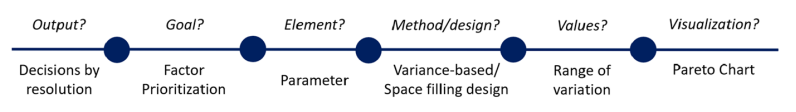
\includegraphics[width = \textwidth]{tex/pics/borgonovo_protocol.png}
    \caption{The six steps for sensitivity analysis of ABMs, adapted from \textcite{Borgonovo2022SensitivityAO}.}
    \label{fig:borgonovo_protocol}
\end{figure}

\begin{enumerate}
    \item \textbf{Choosing the output (or the outputs) of interest.} Depending on whether the model is deterministic or stochastic, the quantity of interest could be the output of the model itself or, if that is a distribution, one of its summary statistics. 
    \item \textbf{Deciding the goal of the sensitivity analysis to pursue (i.e. setting).} The researcher may want to increase their understanding of the model dynamics or to produce insights for the decision-makers. Possible settings have been described above in Section \ref{sa_settings}.
    \item \textbf{Selecting the elements of the model to vary, among parameters and procedures.} The authors propose a conceptual structure for ABMs (graphically represented in \ref{fig:borgonovo_elements}) to classify the "moving parts" of the model that can be subject to sensitivity analysis, among which the researcher is called to pick those they're interested in varying. In particular, the structure distinguishes between two distinct subsets of assumptions, \textit{Parameters} (C) and \textit{Procedures} (E). Parameters are cardinal quantities, characterizing either the agents, the environment or some properties of the simulation; they are determined in advance, before running the simulations, and influence the evolution of the model. On the other hand, procedures are non-cardinal and represent rules of the model or of the simulation; for instance, they could regulate the initialization of parameters or define agents' behavior. The authors propose to \textit{"treat the alternative specifications of a non-parametric element as the levels of a categorical variable"} and to conduct the sensitivity analysis by considering a full factorial design. 
    \item \textbf{Choosing the most appropriate methods to perform the sensitivity analysis for the goal-element-model combination.} Once the goal and the elements of interest have been defined, one has to decide the scale of the analysis (local or global) and, consequently, the methods to adopt. 
    \item \textbf{Assigning numerical values to the parameters of the model.} If the scale of the analysis is local, then the researcher defines the values of the base case and those of one or more alternative scenarios. In case of a global probabilistic analysis, instead, the analyst specifies the support and the distributions of each input of interest.
    \item \textbf{Selecting the appropriate visualization tools to present the results of the analysis.} Choosing the wrong visualization tool may result in a non-effective communication of the results to the stakeholders that have to make decisions out of the simulation's conclusions. Special care must be taken in case of stochastic ABMs, from which one obtains results in the form of distributions. To deal with changes in statistics of those distributions, in fact, it may be required to conduct statistical significance tests.
\end{enumerate}


\begin{figure}[H]
    \centering
    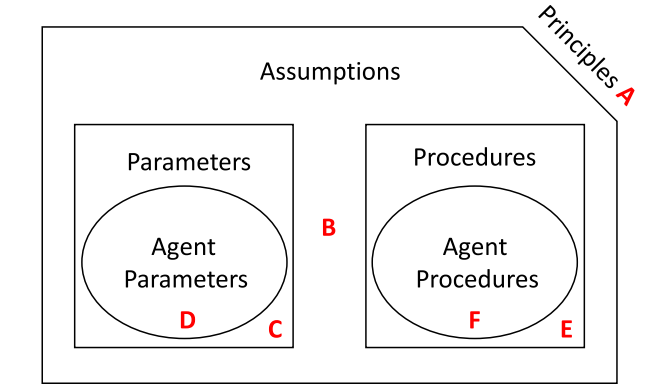
\includegraphics[width = 0.9\textwidth]{tex/pics/borgonovo_elements.png}
    \caption{The four types of elements of an agent-based model, as per \textcite{Borgonovo2022SensitivityAO}: principles, assumptions, parameters and procedures.}
    \label{fig:borgonovo_elements}
\end{figure}


Later, in Chapter \ref{ch:sa}, I will adopt this protocol to perform the sensitivity analysis of an agent-based model for the simulation of traffic flows on Milan's public transportation system, described in detail in Chapter \ref{ch:model}.
\chapter{The Model} \label{ch:model}

% OVERVIEW DEL CHAPTER
In this chapter, I will propose a new Agent-Based Model simulating the mobility of the individuals in Milan that use public transportation services. The model serves the purpose of exploring the consequences of shocks and interventions that directly affect the transport network, allowing decision-makers to plan policies and interventions in a more conscious way. The idea of the model is to reproduce the transport network of the city of Milan as a graph, generate synthetic agents, place them on the graph, and let them move around the city according to their schedules. Individuals interact with each other's as they compete to get on the same vehicle, since vehicles have limited capacity. Moreover, they interact with the environment, since they evaluate all the routes that are available given the current network, and choose the shortest path to their destinations, according to network-specific attributes (i.e. distance between stops, speeds of the vehicles, lines' timetables). 

The proposed model is characterized by four elements:
\begin{itemize}
    \item \textbf{The environment:} the public transport network of Milan, including metro, tram, bus and filobus lines, managed by Azienda Trasporti Milanesi (ATM).
    \item \textbf{The agents:} synthetic individuals, constituting the flow of passengers on ATM vehicles.
    \item \textbf{The time:} the model is designed to reproduce a 20-hour period in an ordinary week day, typically from 5:00 a.m. to 1.00 a.m. of the next day, the time range in which people move using public transports, although it is possible to model longer or shorter periods. Each step represents 1 minute (for a total of 1200 steps in the default setting).
    \item \textbf{The rules:} agents, according to their schedules, move on the network, respecting the timetables and the availability in terms of capacity on the vehicles.
\end{itemize}

In Section \ref{sec:3.1}, I will describe the main data sources I used to build the model and how they have been manipulated. Then, in Section \ref{sec:3.2}, I will explain in detail how the graph representing Milan's transportation system has been constructed. Section \ref{sec:3.3} is devoted to describing the process of synthesizing the agents, as to produce a sample which is the most representative of Milan's population of residents. Finally, in Section \ref{sec:3.4}, I will outline the rules of the model, and, in Section \ref{sec:3.5} I will present some experiments that have been conducted, to show its potential applications.

%%%%%%%%%%%%%%%%%%%%%%%%%%%%%%%%%%%%%%%%%%%%%%%%%%%%%%%%%%%%%%%%%%%%%%%%%%%%%%

\section{Data sources}\label{sec:3.1}
The model is constructed upon data coming from different datasets describing Milan's transportation network and population. We can distinguish between those needed to build the transport network and those used in the process of synthesizing the population, and highlight the main steps of the manipulation process.\\ \\
The datasets used to build the network are the following:
\begin{enumerate} 
    \item Two datasets \cite{site1, site5} from Comune di Milano's open data, containing the main features characterizing each route of the underground lines and of the surface transit lines respectively: an id number, the mean of transport, the line, the terminal points and their geographical coordinates, the length and the number of stops. Here, a line can have multiple routes, active in different time ranges.  
    \item Two datasets \cite{site2, site6} from Comune di Milano's open data, containing the AMAT\footnote{Agenzia Mobilità Ambiente e Territorio, an agency, present in the municipality of Milan, that provides services to support the municipal functions in the fields of planning, programming, management, monitoring and control relating to the development of the territory and greenery, urban planning, mobility and transport public \cite{site21}.} id, the line name and number, the geographical coordinates and the location of all the stops of the metro lines and of the surface transit lines respectively.
    \item Two datasets \cite{site3, site7} from Comune di Milano's open data, containing the sequence of stops for each route of the underground lines and of the surface transit lines respectively;
    \item Two datasets \cite{site4, site8} from Comune di Milano's open data, containing the starting time, the ending time, the type of day (weekday, holiday, weekend) for each route of the underground lines and  of the surface transit lines respectively. 
    \item Datasets \cite{site12} of GTFS\footnote{General Transit Feed Specification, common format for public transportation schedules and associated geographic information.} containing, for each stop, the transit times of all the means of transport, according to the timetables for ordinary weekdays. 
    \item Dataset mapping each stop, defined by the couple of its geographic coordinates, to the NIL\footnote{Nuclei d'Identità Locale, partition of the territory of Milan, introduced in the PGT (Piano di Governo del Territorio).} it belongs to, obtained from an open interactive web-map of Milan \cite{site22}.
    \item Dataset of OpenStreetMap containing information about the geographic area of Milan and the main points of interests.
\end{enumerate} 
I discard routes running only on weekends and holidays and, for each of the remaining routes, obtain the couples of ordered stops representing its sequence. From the OpenStreetMap file (data source 7), I derive the complete list of the points of interest that are present on Milan's territory. I consider only points of interest of selected types, which are categorized into 'amenity', 'shop', 'school', 'leisure', 'office', as they are the most related to the activities the agents in the model will be performing. \\\\
The datasets used to synthesize the population are the following:
\begin{enumerate}
\setcounter{enumi}{7}
    \item Dataset \cite{site18} from Sistema Statistico Integrato (SiSI) of Milan, containing the distribution of resident people in Milan in 2021 by age and by NIL.
    \item Dataset \cite{site10} from Istat, containing the distribution of individuals' movements to perform a specific activity ("\textit{trasporti finalizzati}") by age class during an ordinary weekday (updated to 2013). The population is split in 4 age classes (15-44, 25-44, 45-64 and over 65 years-old) and 7 possible activities are considered.
    \item Dataset \cite{site11} from Istat, showing the average percentage of people performing specific activities by age class in each 10-minute time slot during an ordinary weekday (updated to 2013). Only 6 possible activities are considered.
\end{enumerate}
First, I adapt the different distributions, as to have the same 4 age classes in each of them. I discard the activity "volunteering", of which I only have the distribution of movements but not the information about the proportion of individuals performing it during the day, and I standardize the distributions accordingly. The final list of activities I consider is the following: sleep/eat/personal care, education, family work, paid work, free time\footnote{The names of Istat categories in the original dataset are in Italian, and they are, respectively, "dormire, mangiare e cura della persona", "Istruzione e formazione", "Lavoro familiare", "Lavoro retribuito", "Tempo libero".}. Finally, I rescale each probability of performing a specific activity at each time slot by the proportion of people traveling 40 minutes earlier, 40 being the average duration of daily public transit usage in Milan \cite{bib2}. The intuition is that I want the probability of each age class carrying out a specific activity in a given time slot to be higher if a greater proportion of individuals of that given class were traveling 40 minutes before the given time slot.

%%%%%%%%%%%%%%%%%%%%%%%%%%%%%%%%%%%%%%%%%%%%%%%%%%%%%%%%%%%%%%%%%%%%%%%

\section{The Network}\label{sec:3.2}

Data sources 1 to 4 are combined to construct a directed multigraph, that is a directed graph allowed to have parallel edges connecting the same source and target nodes, representing the public transport network of Milan: each node identifies a stop, while an edge between two stops denotes the existence of a route, of any transportation mean, connecting them. In this way, two consecutive stops on the same transport line are joined by an edge. All the edges point in a single direction, and between two nodes there may be multiple links of different types. In our specific case, this happens when there are two or more routes that pass through two consecutive stops. I only consider the routes that are active during weekdays.

To compute the distances and better visualize the network, all the stops are placed and plotted in the space using their real geographic coordinates, available in data source 2.  
I add to the network several edges representing walking paths connecting those stops that are not linked through transportation means but are close enough to be reached on foot from one another. The introduction of these additional edges allows to obtain a connected graph, a graph with only one component, which, in practice, gives agents the possibility to potentially find a path from any stop to any other one. In the original version of the model, two stops are defined as "at walking distance" if the geodesic distance between them is of maximum $r_{foot}$ = 200 meters. The final graph, including transport means and walking paths, is shown in figure \ref{network_complete} and contains a total of 4753 nodes and 18470 edges. 

Both nodes and edges have been endowed with several attributes.
Each node is characterized by a unique id, which corresponds to the stop's official AMAT id and serves as unique identifier of the stop. For each stop, using data from dataset 7, I compute the number of reachable points of interests corresponding to schools, offices, amenities, and food courts. We say that a point of interest is reachable if its distance from the stop is less than or equal to a number $r_{pois}$, which in the original version was set to correspond to 500 meters. One can think of the points of interest as lying within the ball, centered at the stop, with radius equal to $r_{pois}$.  
 
Each edge is uniquely identified by the 3-tuple containing the ids of the two nodes that it connects and the specific line of the mean of transport it represents (e.g. 11497, 11500, TRAM12). Its attributes are: transport mode, total capacity, weight, next edges, waiting list and passengers list. The total capacity, as per \cite{site13,site14,site15,site16}, and the weight depend on the transport mode. In particular, the weight represents the average traveling time between two stops, which is computed by dividing the distance between stops by the average commercial speed of the vehicle \cite{site17}. "Next edges" is a list which, in most cases, contains the single following edge on the same line. However, there are cases in which forks of the line require a single edge to have two “next edges”. Instead, foot edges do not have “next edges”. Finally, the waiting list and the passengers list are created as empty lists, which will be filled during the simulation to allow the identification of the travelers that are waiting for and boarding each vehicle. 

\begin{figure}
    \centering
    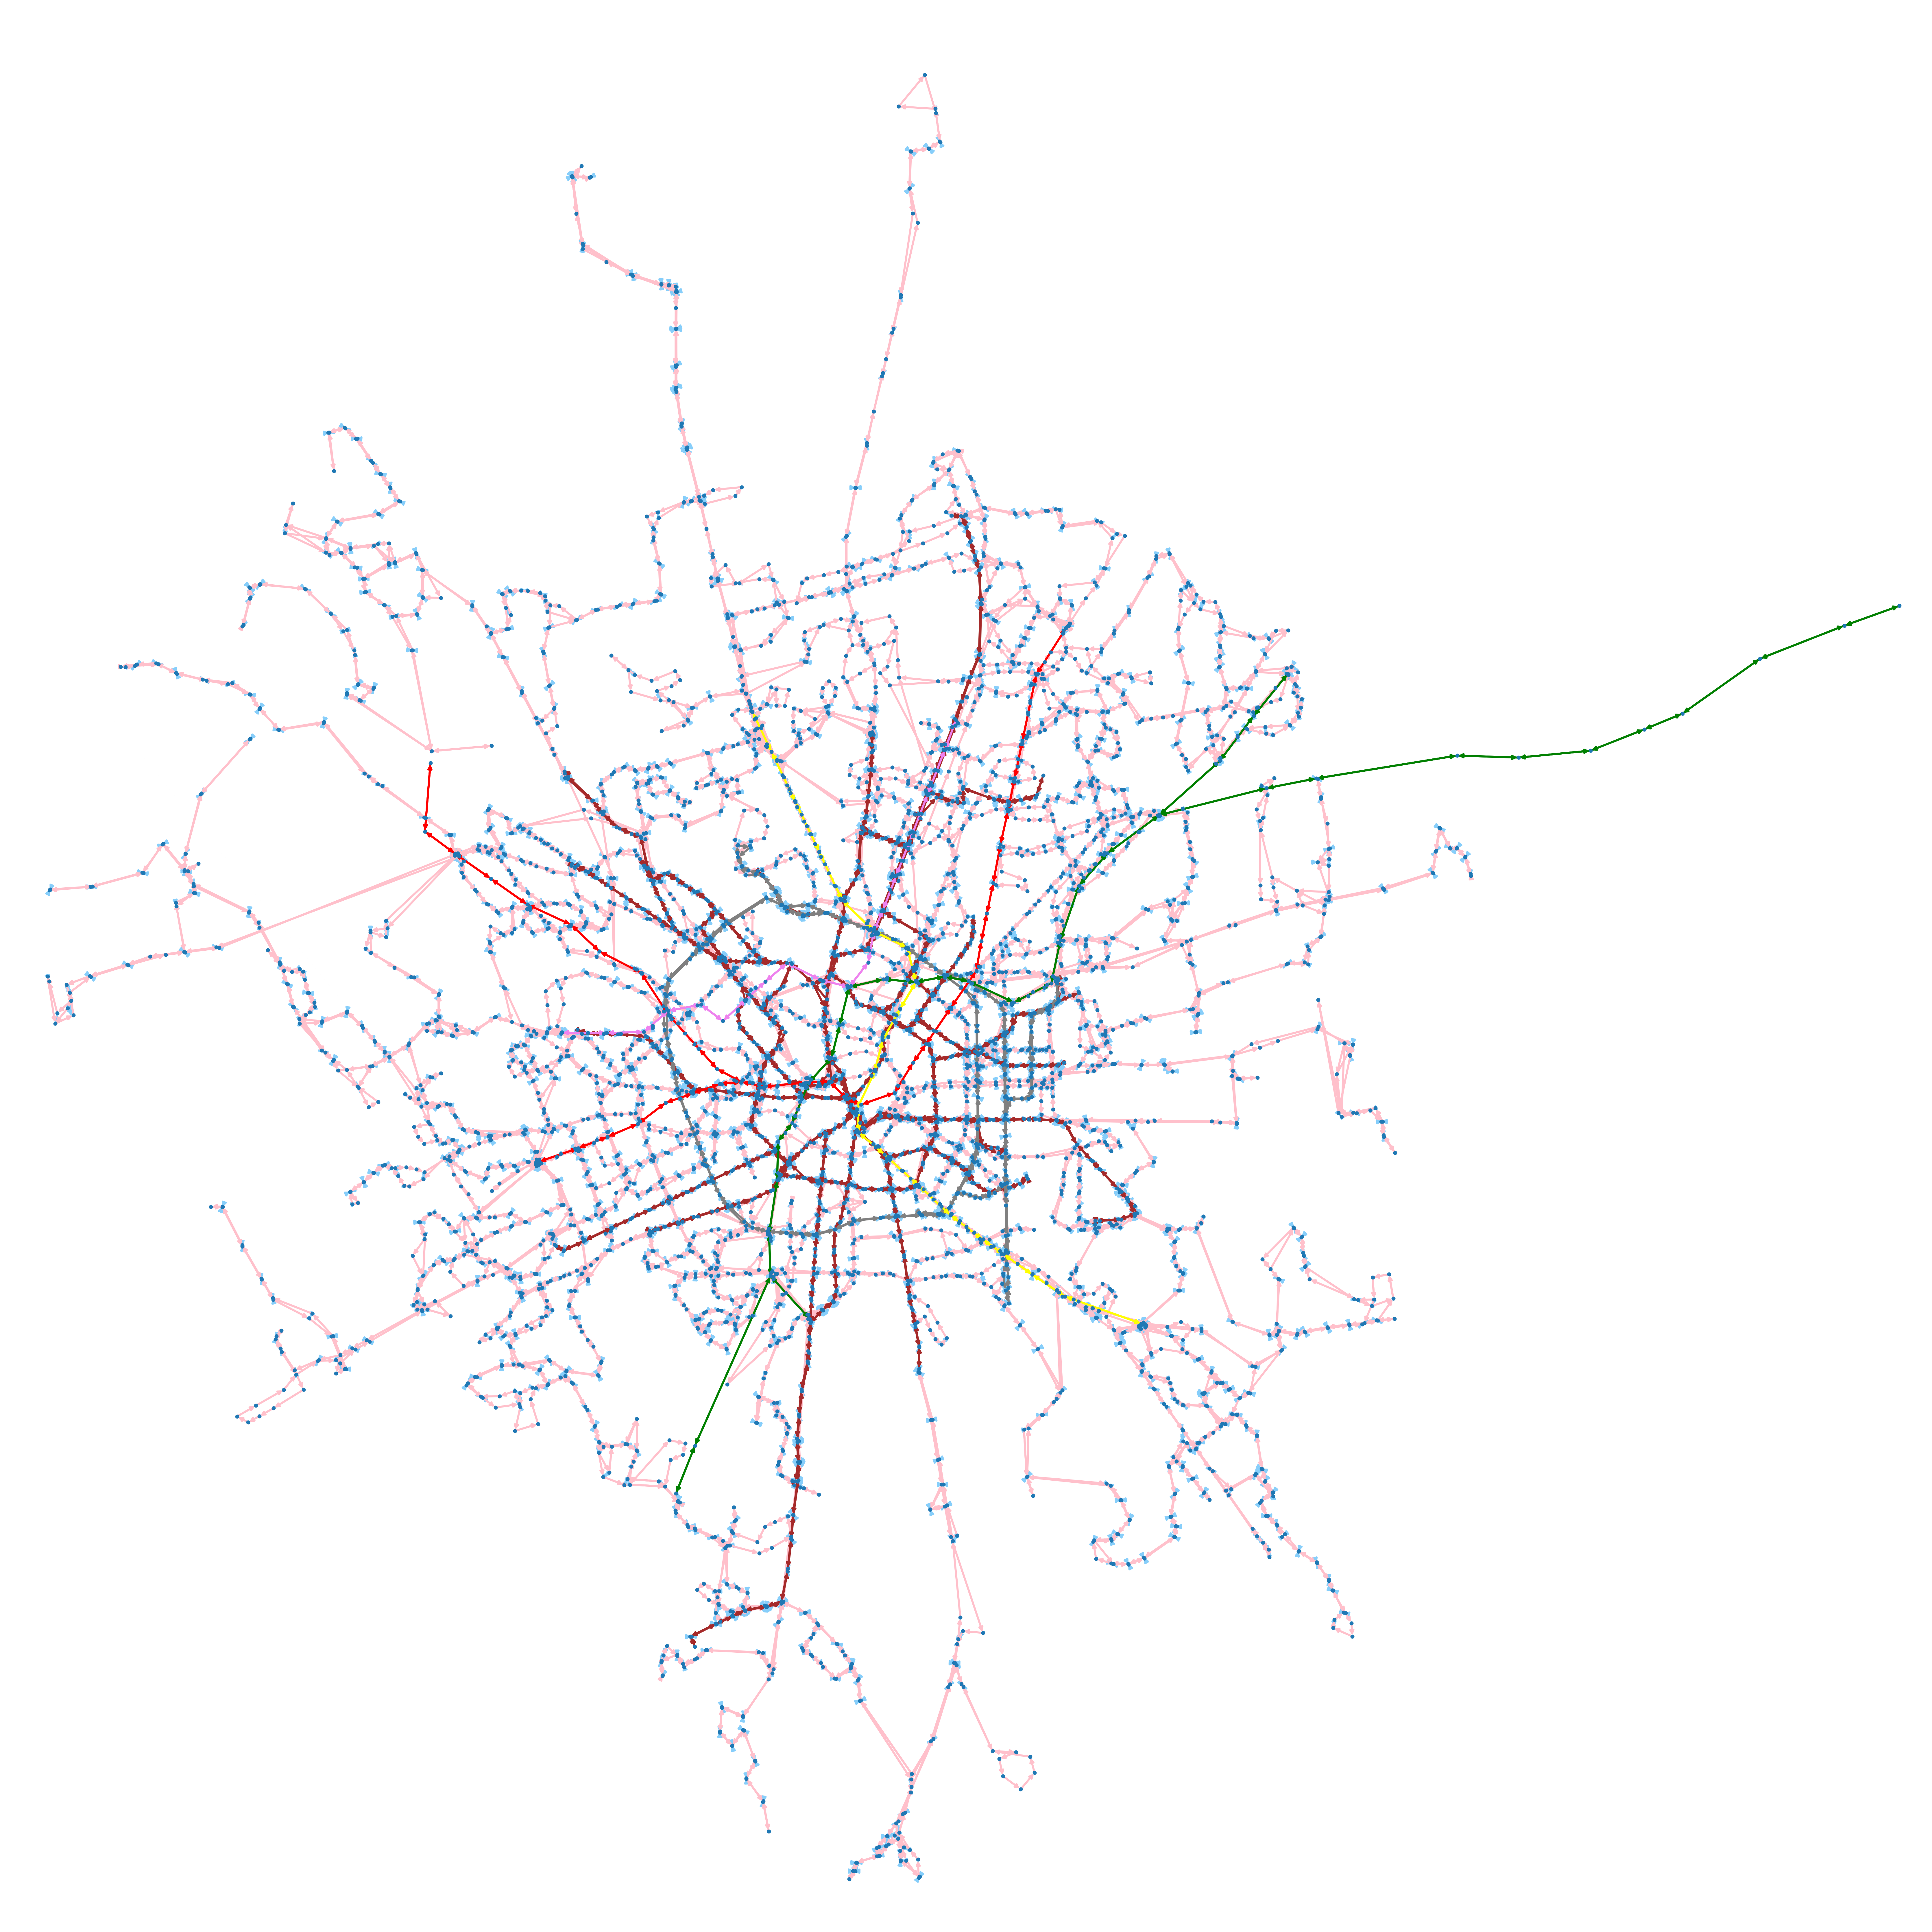
\includegraphics[scale = 0.5]{tex/pics/network_complete_cut.png}
    \caption{The public transportation network of Milan. Different transportation means are represented with different colors: metro line 1 is in red, metro line 2 in green, metro line 3 in yellow, metro line 5 in violet, tram in brown, bus in pink and filobus in gray. Walking paths, for ($r_{foot} = 200 m$), are shown in light skyblue.}
    \label{network_complete}
\end{figure}

%%%%%%%%%%%%%%%%%%%%%%%%%%%%%%%%%%%%%%%%%%%%%%%%%%%%%%%%%%%%%%%%%%%%%%%%%%%

 \section{The Agents}\label{sec:3.3}
 
Agents in the model represent the share of Milan's population which, during weekdays, moves around the city using public transports. I assume that the subpopulation of people moving regularly using public transports has the same distribution by age as the total population of residents, which can be found in \cite{site18}, updated to 2021. I only consider individuals that are older than 14 years old, and each agent belongs to one among 4 possible age classes: 15-24 years old ($\approx 11\%$ of the population), 25-44 years old ($\approx 30\%)$, 45-64 years old ($\approx 34\%)$ and over 65 years old ($\approx 25\%)$.
In this model we account for both systematic mobility, meaning the journeys made for study and working purposes, which happen regularly, and non-systematic mobility, namely those trips that take place less regularly and are attributable to reasons like meeting friends, eating out, going shopping or doing personal activities. I rely on Istat data about Italian population's use of time during an ordinary weekday \cite{site14}, updated to 2013. Agents start their daily routine at home, perform from 1 to 5 activities (among education, work, leisure, self-care/eating\footnote{Istat actually provides a category that includes eat, sleep and other self-care. However, given the time horizon I consider (5:00 a.m  to 1:00 a.m), I assume that “sleep” can be neglected.} and housework) and, eventually, go back home. \\

The creation of the synthetic population proceeds through different steps. First, for each agent I draw an age class from the distribution of inhabitants of Milan. Then, I draw a NIL for the agent's house from the distribution of the NILs conditional on the chosen age group \cite{site18}. Finally, I draw, uniformly at random from the stops in the selected NIL, a precise node which represents the agent’s home. 

At this point, two possible strategies can be adopted to assign a travel diary to the agents:
\begin{itemize}
    \item \textbf{Strategy 1.} For each of the five possible activities, I decide whether the agent will or will not perform it during the day, by drawing from a Bernoulli with parameter equal to the probability that the agent carries out such activity in an ordinary weekday, conditional on the agent's age class. Data used to construct this probability distribution come from data source 9. Adopting this strategy, each agent can have a variable number of activities to carry out, ranging from 1 to 5. The strategy is summarized in the algorithm \ref{alg1} below.
    \item \textbf{Strategy 2.} Agents are forced to perform a number $k$ of activities. The combination of activities to perform is drawn with replacement from the distribution of possible combinations conditional on the age group the agent belongs to. Specifically, I consider the choices of activities as independent of each other, so that the conditional probability of each combination corresponds to the product of the conditional probabilities of the single activities in it. The strategy is summarized in the algorithm \ref{alg2} below.
\end{itemize}
In the original version of the model, strategy 1 has been adopted. On average, using strategy 1, around $20\%$ of the initially generated agents come with no planned activities in their schedule and, therefore, are discarded. Experiments show that agents' schedules only contain 2 activities on average. To make the results of the two strategies comparable in terms of traffic load on the network, the parameter k for the second strategy will be set to 2 by default for following experiments. 

\begin{algorithm}[h!]
\caption{Agents' generation - strategy 1}\label{alg1}
\begin{algorithmic}
\Require $n \geq 0$
\For {each agent $i = 1, ..., n$}:
\State $\textit{age\_class} \sim Multinomial(p_l)$ \Comment{$p_l$ = P(age class l) for $l = 1, ..., 4$}
\State $\textit{nil} \sim Multinomial(q_{jl})$ \Comment{$q_j$ = P(nil j $\vert$ age\_class) for $j = 1, ..., 89$}
\State $\textit{home} \sim Uniform(k)$ \Comment{$ k = \frac{1}{\vert \{s: s \in nil \} \vert }$}
\For {each activity a = 1, ..., 5}:
\State $ \textit{u} \sim Bernoulli(f_a)$ \Comment{$f_a$ = P(a $\vert$ age\_class)}
\If{$u = 1$}:
    \State $\textit{destination} \sim Multinomial(g_s)$ \\\Comment{$ g_s = \frac{ \# \text{ amenities of type a close to node s}}{ \# \text{ total of amenities of type a}}$}
    \State $\textit{departure\_time} \sim Multinomial(r_t)$ \\\Comment{$r_t$ = P(travel time $\vert$ a) + U(-5, 5)}
\EndIf
\EndFor
\EndFor
\end{algorithmic}
\end{algorithm}

\begin{algorithm}[h!]
\caption{Agents' generation - strategy 2}\label{alg2}
\begin{algorithmic}
\Require $n \geq 0$
\For {each agent $i = 1, ..., n$}:
\State $\textit{age\_class} \sim Multinomial(p_l)$ \Comment{$p_l$ = P(age class l) for $l = 1, ..., 4$}
\State $\textit{nil} \sim Multinomial(q_{jl})$ \Comment{$q_j$ = P(nil j $\vert$ age\_class) for $j = 1, ..., 89$}
\State $\textit{home} \sim Uniform(h)$ \Comment{$ h = \frac{1}{\vert \{s: s \in nil \} \vert }$}
\State \textit{activity\_combination} $\sim Multinomial(\theta_c)$
\\\Comment{$\theta_c$ = P(combination c $\vert$ age\_class) for $c = 1, ..., \binom{5+k-1}{k} $}
\For {each activity a = 1, ..., k in activity\_combination}:
\State $ \textit{u} \sim Bernoulli(f_a)$ \Comment{$f_a$ = P(a $\vert$ age\_class)}
\If{$u = 1$}:
    \State $\textit{destination} \sim Multinomial(g_s)$ \\\Comment{$ g_s = \frac{ \# \text{ amenities of type a close to node s}}{ \# \text{ total of amenities of type a}}$}
    \State $\textit{departure\_time} \sim Multinomial(r_t)$ \\\Comment{$r_t$ = P(travel time $\vert$ a) + U(-5, 5)}
\EndIf
\EndFor
\EndFor
\end{algorithmic}
\end{algorithm}

I assign a location to each activity selected for the agent (i.e. the specific node in the network) with probability proportional to the number of facilities corresponding to that task that are located nearby each node \cite{site9}. Among the possible categories proposed by OpenStreetMap, I only take into consideration the ones that match Istat activities (eg. schools, universities, etc. for education; offices, co-working place, etc. for work; cinema, gyms, etc. for leisure time; restaurants, bars, etc. for eat/sleep). When the activity “housework” is selected, I assign as destination of the trip the node corresponding to the agent’s house. I then appoint a departure time to each scheduled activity by drawing a 10-minutes time slot from the distribution of oriented movements over time, conditional on the specific activity \cite{site11} shifted back by 40 minutes, as I assume the activity will be performed approximately 40 min after the departure (40 minutes being the average traveling time according to \cite{bib2}). To allow for minute-by-minute departure times, I also include a randomization term that adds or removes at most 5 minutes from the picked time. 

Finally, if the last destination of the agent is not “home”, I compute a critical time at which the agent will depart again to go back home (time of the last activity + 40 min + average duration of last activity + noise in the [-10 min, +10 min] interval). I consider two possible sets of average duration for the activities:
\begin{itemize}
\item set 1: 120 min for sleep/eat/personal care, 330 min for education, 440 min for paid work and 90 min for free time;
\item set 2: 120 min for sleep/eat/personal care, 156 min for education, 220 min for paid work and 90 min for free time.
\end{itemize}
The numbers in the first set have been computed by averaging across age-classes the duration of activities from Istat data in \cite{site11}. In set 2 the average duration of education and paid work have been reduced by 50\%, as to allow for part-time occupations. 
The set used to compute the critical time is randomly chosen, for each agent, through a Bernoulli draw with parameter $p_{long}$ equal to the probability of choosing set 1 (the one with the longest average duration of activities). I set $p_{long}$ to 0.7 if the time of the last activities is before 1.30 a.m. and to 0.3 if it is after, as I believe that there is a higher chance of performing a long activity if that is started in the morning rather than in the second part of the day.
I assume that, if this critical time is after 10:30 p.m. the agent prefers not to use public transports to go back home, as the timetables are not favorable later in the evening. 


At this point, for each agent we have: a unique id, the age group, the starting point (node on the network) and a schedule of activities (from 1 to 5 activities, with the related destination and the time at which the agent has to start the journey to get there), as in the example in table \ref{tab1}. 


\begin{table}
\centering
\caption{Example of agent's generation}\label{tab1}
\begin{tabular}{ll|lll}
\multicolumn{2}{c|}{The agent} & \multicolumn{3}{c}{The schedule} \\ 
\toprule
Features      & Data      & Activity & Destination & Departure time \\ 
\midrule
Unique id & 7548 & 1) Education & V.le Bligny, 19 & 7:30\\
Age & 15-24  &  2) Work	& Duomo M3 & 14:15\\
Starting point & Corvetto M3 & 3) Leisure & Moscova & 19:25\\
\bottomrule
\end{tabular}
\end{table}

The final step to complete the synthesis of the population is to assign to each agent the list of edges that form the shortest path they will use to reach their destinations. Specifically, the shortest path is calculated through the Dijkstra algorithm, using as weight for each edge its traveling time. However, not all nodes are taken into account in this process. In fact, the shortest path is computed on the subgraph of the edges constituting the transportation lines that are active in a limited time window around the departure time. In this way, the agent can only select routes that are available at the time of their departure. This means that two agents who have been assigned the same couple of departure and destination stops may take two different paths to reach their common destination if the trips are scheduled at different times during the day. Lastly, since I am working on a multigraph, it may be the case that two stops are linked by two different means of transport with same speed. In this case, the agent includes in the shortest path the edges that minimize the number of changes of vehicles needed. \\


Agents are characterized by a state, which can take four possible values: busy, waiting, traveling and finished. Busy agents are those that are currently in one of the facilities and do not have to travel. Waiting agents are the ones waiting at a stop in order to get on a vehicle. Traveling agents are situated on edges, and they are moving to their next destination. Finally, finished agents are those that have already completed all the journeys in their daily schedule. 

%%%%%%%%%%%%%%%%%%%%%%%%%%%%%%%%%%%%%%%%%%%%%%%%%%%%%%%%%%%

\subsection*{Validation of the synthetic population}\label{ssec:3.3.1}

Although the synthesis of the population is stochastic, as it involves multiple draws from different distributions of demographic and geographical features, choosing a large sample size allows to obtain samples of synthetic agents which resemble the true population. I estimate that the individuals take, on average, 8 different vehicles during the day: counting each time an agent takes a different vehicle as a separate passenger, if I start with 20000 agents then I get a total of 160000 synthetic passengers per simulation. If I treat each of them as representing 10 real people, and adjust vehicles' capacities accordingly, then I am able to run a simulation that represents the whole population of daily travelers on all the transport network of Milan, which amounts to 1590000 people, as reported in \cite{site20}. A sample size of 20000 agents is believed to be large enough to achieve low variability of agents' characteristics across different samples. To demonstrate this, I have generated 100 samples of 20000 synthetic agents, observed the distributions of multiple characteristics and computed means and standard deviations. The reported bar charts show that the observed distributions don't deviate significantly from the true ones. Numerical values for the means and standard deviations are available in the \nameref{appendix}.
One can easily see that the true relative proportions of age classes are preserved, with low standard error, as shown in figure \ref{pop_age}. Similarly, the estimated relative proportions of the population resident in each NIL resemble the true distribution, as shown in figure \ref{pop_nil_tot}. Details about the distribution of the population by NIL conditional on age classes are reported in the \nameref{appendix}. The last distribution observed is that of the combinations of activities performed by agents, under assignment strategies 1 and 2. The bar charts in figures \ref{pop_act} and \ref{pop_act2} show, on the left, in blue, the weighted average of the probabilities of the different combinations of activities, with weights equal to the proportions of the four age classes, and, on the right, in orange, the observed number of individuals per combination, averaged across samples. It is easy to see that variability across samples is low in both cases, and the observed proportions resemble the sampling distributions.

\begin{figure}
    \centering
    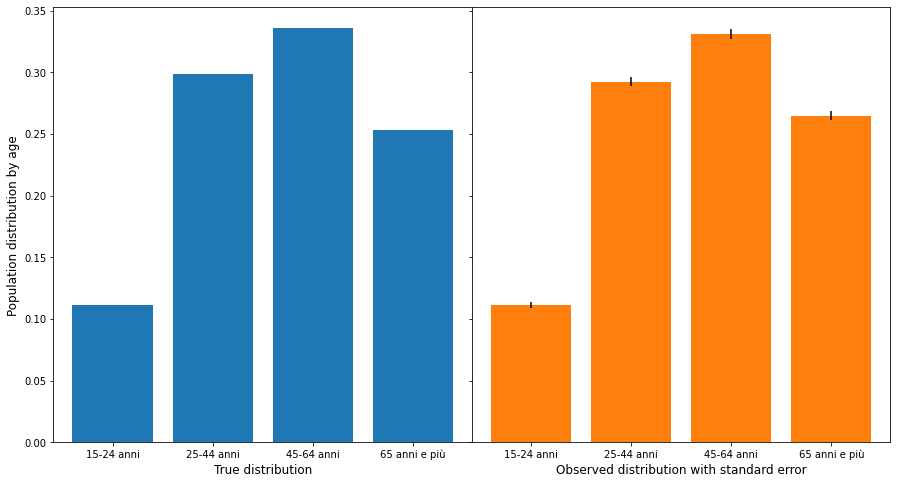
\includegraphics[scale = 0.5]{tex/pics/pop_by_age.png}
    \caption{Comparison between the true population distribution by age (in blue) and the observed one (in orange) with standard error, averaged across 100 samples.}
    \label{pop_age}
\end{figure}

\begin{figure}
    \centering
    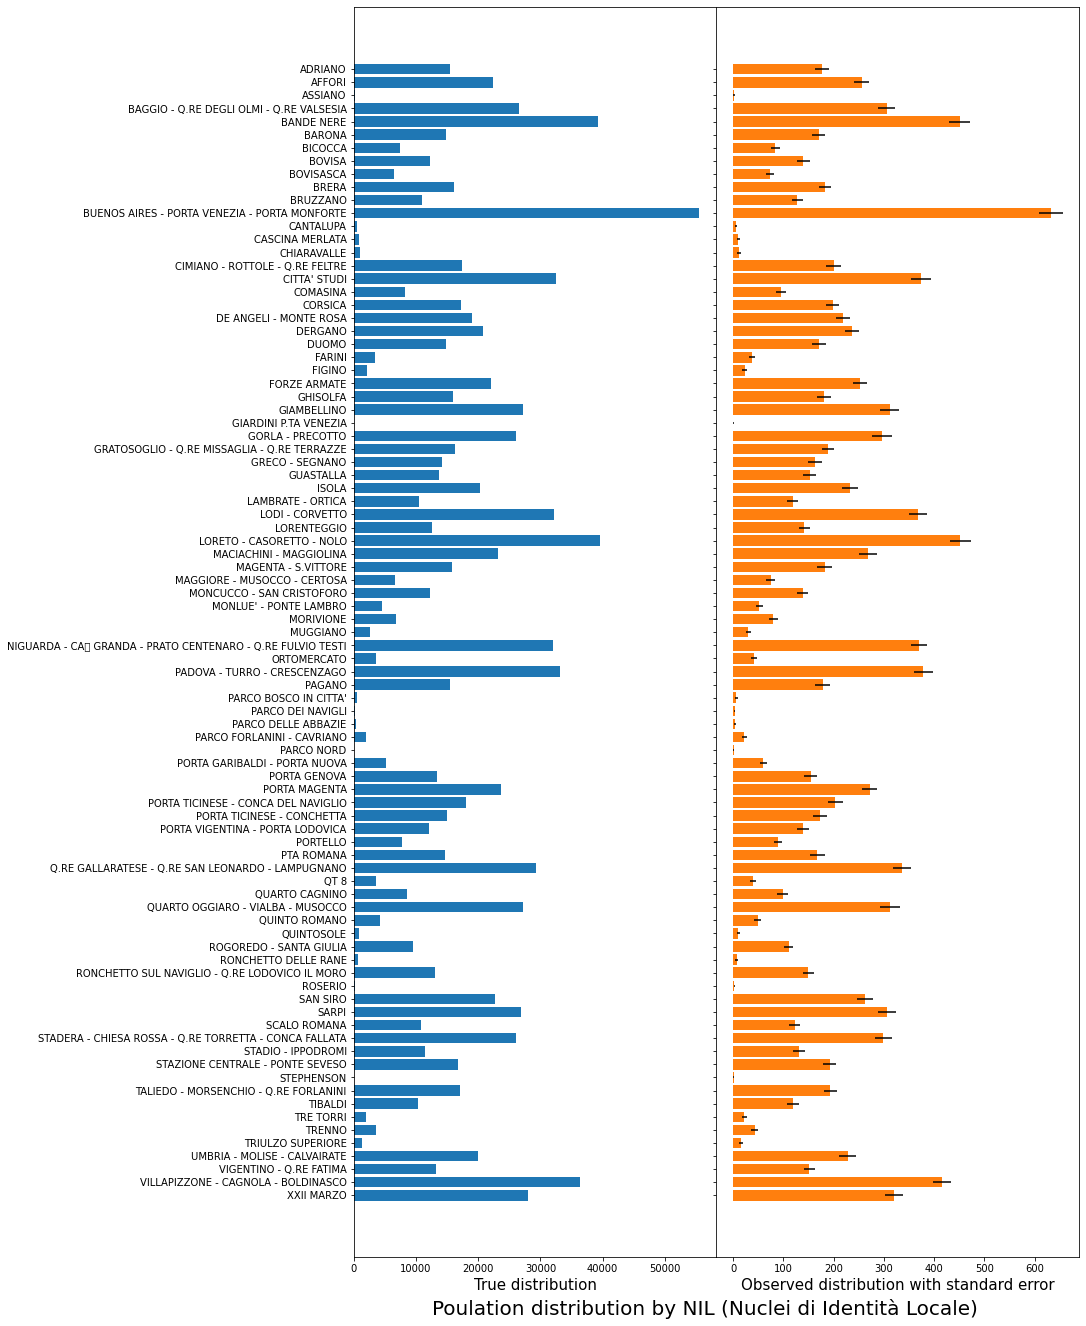
\includegraphics[scale = 0.45]{tex/pics/pop_by_nil_tot.png}
    \caption{Comparison between the true population distribution by NIL (in blue) and the observed one (in orange) with standard error, averaged across 100 samples.}
    \label{pop_nil_tot}
\end{figure}



\begin{figure}
    \centering
    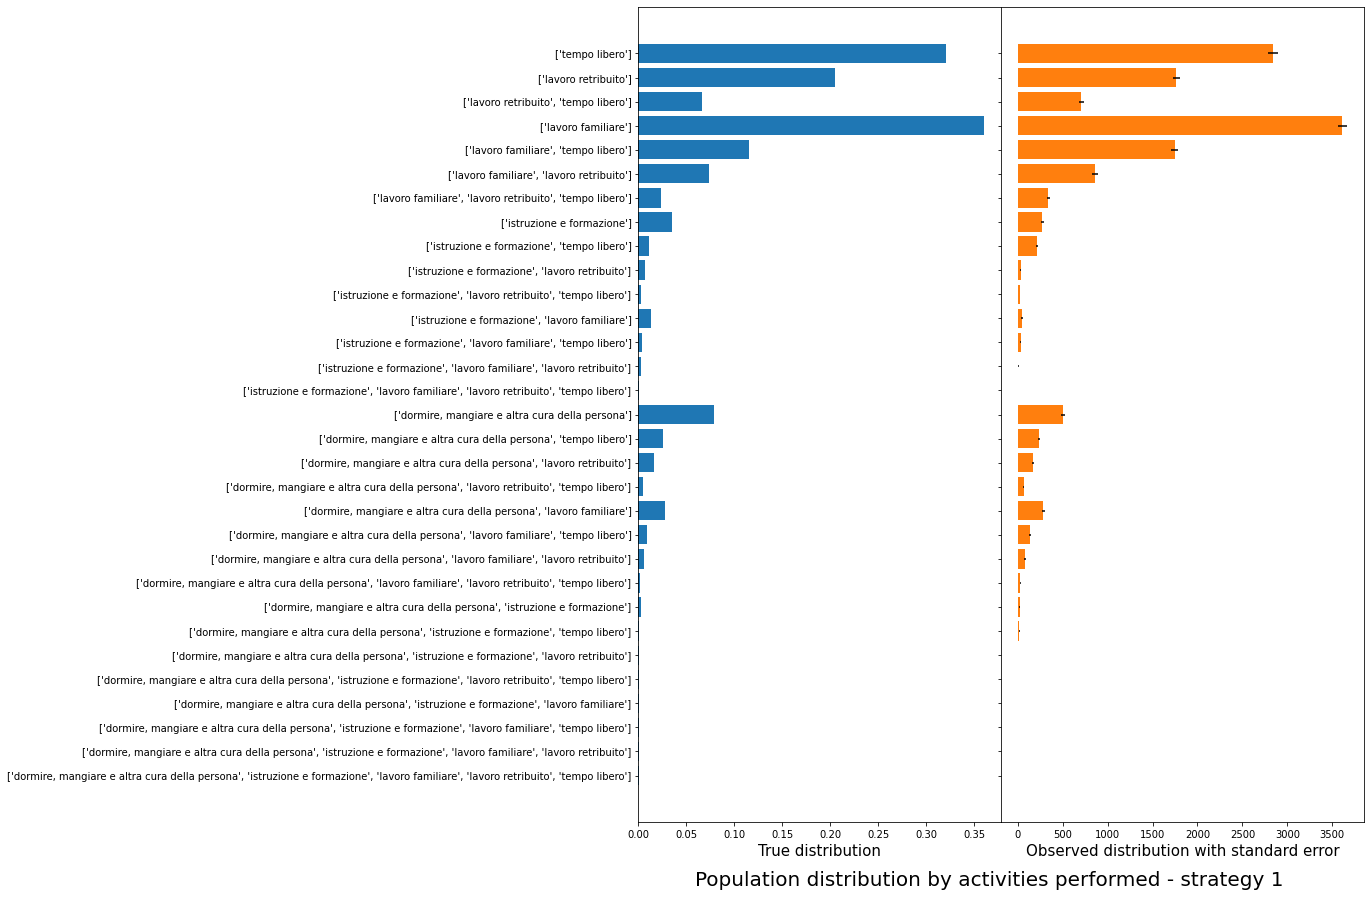
\includegraphics[scale = 0.35]{tex/pics/pop_by_act.png}
    \caption{Comparison between the true population distribution by activities performed (in blue) and the observed one (in orange) with standard error, averaged across 100 samples. Strategy 1 is used to assign activities to agents.}
    \label{pop_act}
\end{figure}

\begin{figure}
    \centering
    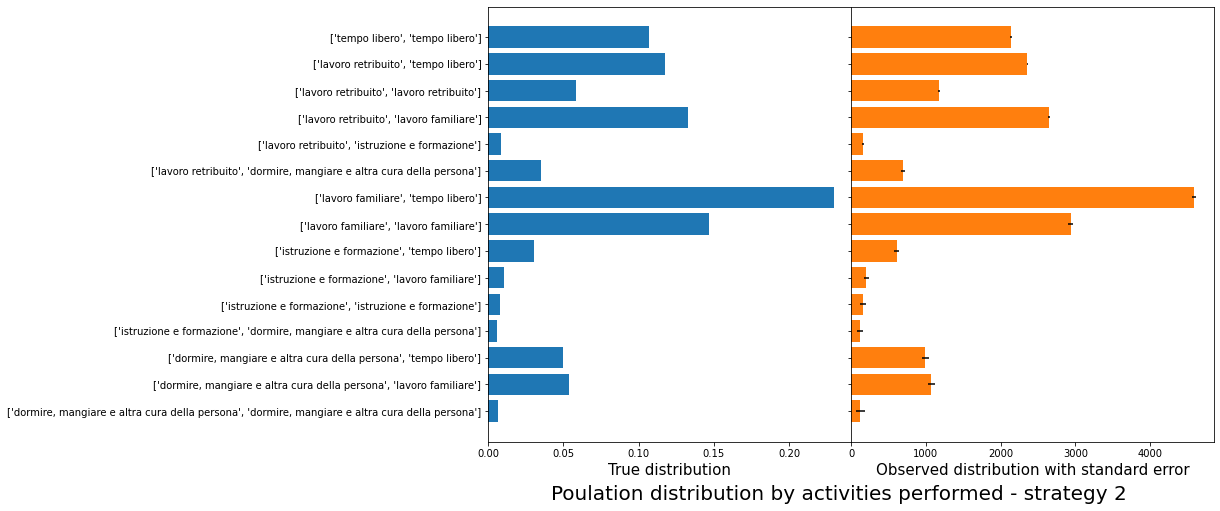
\includegraphics[scale = 0.4]{tex/pics/pop_by_act2.png}
    \caption{Comparison between the true population distribution by activities performed (in blue) and the observed one (in orange) with standard error, averaged across 100 samples. Strategy 2 is used to assign activities to agents.}
    \label{pop_act2}
\end{figure}

%%%%%%%%%%%%%%%%%%%%%%%%%%%%%%%%%%%%%%%%%%%%%%%%%%%%%%%%%%%%%%%%%%%%%%%%%%%

\section{The Rules}\label{sec:3.4}

Once the population of agents has been synthesized, all agents are initialized to the busy status and let move on the network to reach the destinations in their schedule. 
The typical simulation reproduces 20 hours, from 5:00 a.m. to 1:00 a.m. of the next day, but start and end time can be customized.
Each iteration of the simulation represents one minute. At each minute, I activate agents within groups in random order, to avoid giving the first-mover advantage to the same individual at each timestep. I first consider the set of “busy” agents: if they are scheduled to depart at the current minute, their status changes to “waiting”, otherwise, they remain “busy” at their current position. I then loop over the “traveling” agents: looking at their path, they evaluate whether they have to get off the current vehicle and disembark if that is the case. Clearly, they can only do so if the vehicle has gone across the edge and reached the next stop. Edges in the graph can be either active or inactive at any given time step: an edge is active at minute t if there’s a vehicle that is stopping at the starting node of the edge and can embark passengers. “Waiting” agents are the last to act: each of them looks at the next edge in their path and, if it is active and there’s space on the vehicle, they get on board, while, if that is not the case, they stay on the stop waiting for the next activation. Once an agent completes all of its tasks, its status changes to “finished” and it is no longer considered in the following iterations. It can happen that agents are scheduled to depart for an activity very late in the night, when rides are less frequent, so they fail to complete their journey, and their status never becomes “finished”. I assume that, in this case, they will use alternative ways, not covered in our model, to proceed. \\

Now that we have described all the ingredients that characterized the model, we can summarize it by mapping its elements into the sets presented by Borgonovo et al. in \cite{Borgonovo2022SensitivityAO}:
\begin{itemize}
\item \textbf{Principles:} a principle of the model is that agents' houses are exactly on transport lines' stops. Indeed, the environment in this model is a network made of the points identifying stops and the lines connecting them, not the continuous Euclidean space representing the surface of Milan. This simplification seems reasonable, as I assume that the path from agents' houses to the closest stop is negligible. Hence, we can think of the departure times as the times at which an agent will be at the stop, ready to embark on a vehicle, rather than the times at which they plan to live their houses (or, more in general, their location). Another principle of the model is the characterization of agents through a state taking 4 possible values: busy, waiting, traveling and finished. A state determines the behavior of an agent in future steps. Making changes to the states system, for example as to allow for other admissible values for agents' state, would lead to a different model. 
\item \textbf{Assumptions:} an assumption of the model is that agents move on the environment representing the network of public transports of the city of Milan and have full knowledge of the network, so that they are able to plan in advance the path to follow in order to minimize traveling time. The current version of the network is built on data updated to 05/05/2022. Any update to the routes would result in a different version of the network, but that would not change the essence of the model. Similarly, one can adapt the model to a different city just by changing the network and timetables, if no modifications to the rules are made. I assume that agents are not aware of lines' timetables: they compute traveling time and base their choice of path on the assumption that the vehicles will be immediately available at the stop when they arrive.
\item \textbf{Parameters linked to the environment:} two important parameters of the environment are the capacity and speeds of vehicles, that determine the weights of edges and, hence, the expected traveling time agents consider when deciding which path to follow. Another important parameter is the maximum distance used to consider two stops as "at walking distance" ($r_{foot}$). This is crucial as it dictates the number of fictitious "foot" edges added to the original network and, consequently, the total number of possible paths available. Finally, one last parameter is $r_{pois}$, which I use to compute the number of points of interests that are reachable from each stop. This parameter plays an important role as it changes the probabilities of each activity being performed in proximity of any stop.
\item \textbf{Agents' Parameters:} the number of age classes and of possible activities the agents can perform are important parameters characterizing agents' profiles. The distributions of the age classes and of NILs given age class are multinomial distributions whose parameters need to be mentioned among agents' parameters. Moreover, the probability of agents performing "long" tasks rather than short ones, $p_{long}$, is an important parameter which influences agents' decision to return back home with public transports at the end of their schedule.
\item \textbf{Procedures:} some procedures describe the way in which agents are able to embark vehicles: first traveling agents get off, then waiting agents try to get on in random order, succeeding unless full capacity of the vehicle is reached. Another relevant procedure is the strategy used to sample activities: the standard one is to allow for one possible occurrence of each activity during the day, while, an alternative is to allow for repetitions of each activity up to a number k of total activities. 
\end{itemize}

%%%%%%%%%%%%%%%%%%%%%%%%%%%%%%%%%%%%%%%%%%%%%%%%%%%%%%%%%%%%%%

\section{Simulation outputs and experiments}\label{sec:3.5}
During the simulation, the researcher is able to collect measures and statistics about the agents, which help evaluate the state of the system and the effects, in terms of flow and overload, of shocks and interventions. 
In particular, interesting KPIs are:
\begin{itemize}
    \item total waiting and traveling time;
    \item total waiting and traveling time per trip;
    \item percentage of traveling and waiting agents at each time step;
    \item total number of vehicle changes;
    \item total number of minutes each edge reaches its full capacity;
    \item total number of times an agent travels on foot;
    \item total number of passengers on each vehicle during the day;
    \item total number of agents passing on each node and each edge;
    \item maximum number of simultaneous agents on an edge (maximum load reached by the vehicle);
    \item distance-adjusted time-per-trip distribution, meaning the distribution of agents by the time it takes for them to cover 1 km.
\end{itemize}

The proposed model allows to test the effects of the implementation of measures already enforced in reality, and to make forecasts about possible scenarios that have not been realized yet, provided that data about the network structure and transport timetables after the changes are available.
Experiments have been conducted to evaluate two realistic scenarios:
\begin{itemize}
    \item \textbf{Suspension of metro stop "Duomo"}, both in metro line 1 and metro line 3. This intervention is usually implemented in Milan when big events, such as concerts or shows, are organized in Piazza Duomo, in order to preserve public security and reduce the affluence to that stop that could be overcrowded: ATM temporarily interrupts the possibility to get out of the Metro 1 and Metro 3 in Duomo, allowing direct connections between the immediately previous and subsequent stops of the metro line.  
    \item \textbf{Introduction of the new metro line 4}, which is expected by the end of 2023. The route comprehends 21 stops, and it aims to connect the western side of Milan, from San Cristoforo, to Linate Airport.
\end{itemize}
In order to account for the uncertainty due to the population synthesis' stochasticity, 10 separate simulations per each phase of each experiment have been run and results have been aggregated. For each experiment, 10 groups of, on average, 20,000 agents have been initialized\footnote{Activity assignment has been conducted adopting strategy 1, which, on average, discards 20\% of agents, having empty schedule. Therefore, to obtain a net sample size of approximately 20000, the number of agents to generate has been set to 25000.}, each one representing 10 real passengers. \\
The experiments consist of two phases, one before and the other after the network changes, in which the same samples of agents are used. The impact of the interventions is evaluated comparing the average waiting time and traveling time before and after the intervention, both for the set of involved agents (those whose paths were affected by the shock) and the whole sample of agents. Moreover, I am able to isolate the most and less impacted lines and also the route sections experiencing the highest load during the day.
\chapter{Sensitivity Analysis} \label{ch:sa}

% - why deterministic
%     --> what is stochastic and why we can treat it as deterministic:
%         - stochasticity in the population synthesis
%         - stochasticity in the boarding priority (negligible)

% - borgonovo protocol
%         - outputs
%         - goal
%         - elements
%         - methods
%         - values
%         - visualization
        
% - visualizations & results & comments vari 


%%%%%%%%%%%%%%%%%%%%%%%%%%%%%%%%%%%%%%%%%%%%%%%%%%%%%%%%%%%%%%%%%%%%%%%%%%%%%%%%%%%%%%%

\section{Preliminaries} \label{sec:ch4_pre}

The first thing to understand in order to set up the sensitivity analysis of an agent-based model is whether the model under study is stochastic or deterministic. Let us recall the difference between the two frameworks: a model is \textit{deterministic}, if by fixing its input, the output remains unchanged when evaluating the model multiple times; alternatively, a model is \textit{stochastic} if it produces a random value any time it is run with the same fixed input. The nature of the model dictates the kind of output one is going to investigate and the course of the analysis to perform. In the case of a stochastic model, one would want to compute descriptive statistics of the conditional distribution of the output given the fixed values of the inputs, and this requires to evaluate a sufficient number of samples, in order to average out the random component in the output, making the analysis more computationally expensive. If the model is deterministic, instead, one simulation run per each value of the inputs is enough to be able to assess the uncertainty in the outputs. \\ So, before diving deep into the analysis, let us briefly recap the model under study in this research, which has been explained in detail in Chapter \ref{ch:model}, to understand its nature and plan the next steps of the analysis accordingly. The idea of the model is to reproduce the flow of passengers using Milan's transportation network, in order to evaluate the efficiency of the system.
\begin{figure}
    \centering
    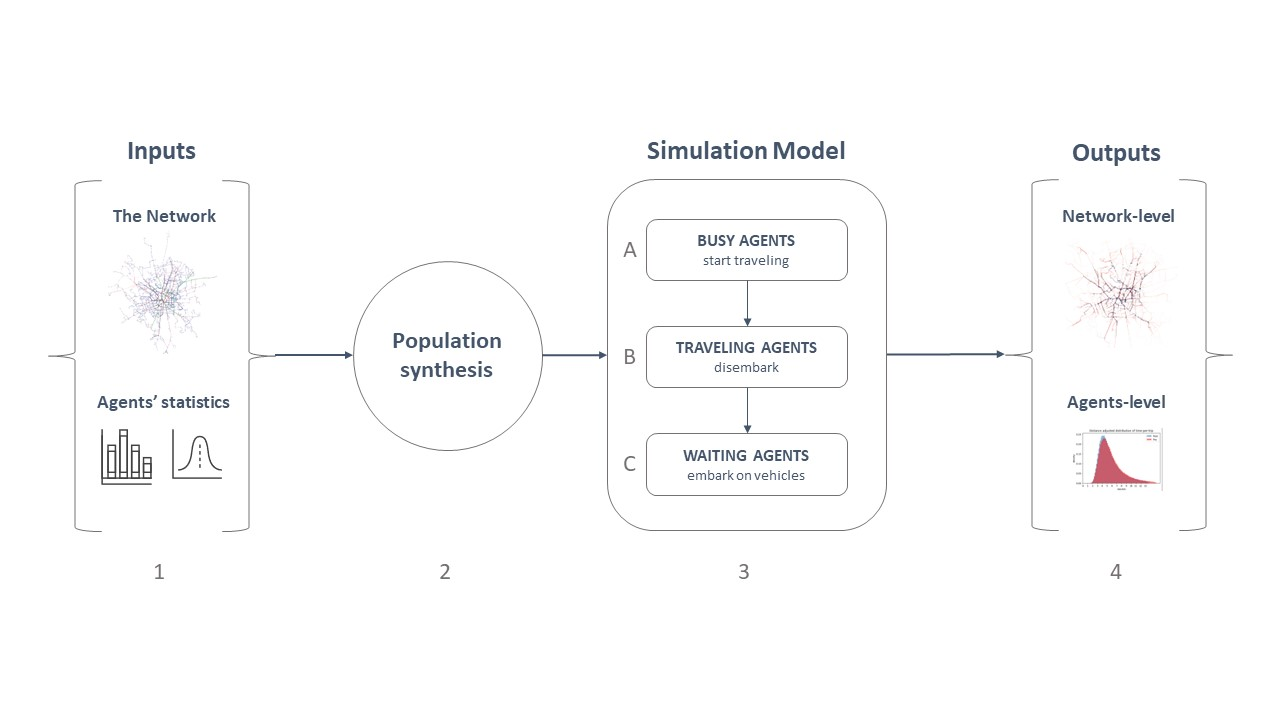
\includegraphics[width = \textwidth]{tex/pics/model_ppt2.jpg}
    \caption{Diagram representing the sequence of steps characterizing the agent-based model under study in this research.}
    \label{fig:model_schema}
\end{figure}
Figure \ref{fig:model_schema} portrays the main phases of the model. On the left side, there are the inputs that need to be fed to the simulator, which can be divided into those needed to construct the network, that will be the environment of the ABM, and those related to the distribution of agents' characteristics. Once one has collected all the inputs, the first step is to run the synthesis of the population. The goal of this phase is to obtain a fictitious population of agents which is as similar as possible to Milan's population, with respect to age, geographical residence and activities performed during an ordinary weekday. Next, the agents obtained are fed, together with the network, to the simulator: as soon as the simulation starts, they begin to move on the network to reach the location of the activities they have to perform. At the end of the simulation, the researcher is able to collect outputs related to the network (e.g. the most overloaded lines) or to the agents (e.g. traveling and waiting time), both at the individual and collective level. 
We can easily recognize two sources of stochasticity in the model's structure:
\begin{itemize}
	\item \textbf{the population synthesis} (2);
	\item \textbf{the boarding priority for waiting passengers} (C). 
\end{itemize}
I will now go through each of the two, in order to show that the impact of their stochastic nature on the model's results is negligible. In other words, for the purpose of the sensitivity analysis, from now on we will treat the model as if it were deterministic, that is, as if we obtain the same identical results from each model run, once the network, the population distributions and the number of agents has been fixed. This would allow us to perform one single run for each parameter setting and make the analysis less computationally expensive.

\paragraph{The population synthesis} 
As described in Section \ref{sec:3.3}, in order to construct the profile of each agent, features like age class, geographical residence and kind of activities performed are drawn from their respective distributions, which have been extrapolated from real demographic data about the residents of Milan. The population synthesis is, thus, a stochastic procedure, producing, at each run, a possibly different sample of agents. The problem with this stochasticity is that agents behavior in the simulations depend on their characteristics. In paricular, the probability of living in a specific zone of the city and that of performing a certain activity are conditional on the age class the agent belongs to, and how busy are agents is among the main drivers of traffic on the network. Moreover, agents' destinations depend on the activity they have to perform, which, again, depends on the age class. In an agent-based models, the results are determined by the collective behavior of agents. Hence, running the simulations with any specific set of individuals would lead to unique results and possibly to the emergence of a distinct phenomenon. For example, in our model, if the number of agents in a sample having the same destination is above average, then the results of the simulation would be biased, as they could show a particular overload on lines that lead to that specific destination. Since one wishes to eliminate, from the bias in the results, the component which depends on the population synthesis, a best practice would be to evaluate the model with multiple batches of agents and then agerage results across simulations. However, one can demonstrate that a large sample size ensures to achieve enough stability in the proportions of the agents' characteristics, across different samples resulting from the population synthesis procedure. That is, if the sample size is large enough, then the empirical distribution of agents will resemble the true distribution and one can decide to treat each sample as if they were equivalent, producing similar results. This kind of analysis can be included in the process of validating the population synthesis, as to assess its robustness. Indeed, in Section \ref{ssec:3.3.1}, I compared 100 samples of synthetic agents, of which I observed the distributions of multiple characteristics. Results show that, with a sample size of 20000, variability across samples is low. Hence, I decide to set default sample size to 20000 and disregard the stochasticity in the agents' profiles creation for the purposes of the sensitivity analysis.

\paragraph{Waiting agents' boarding priority}
As explained in \ref{sec:3.4}, at each timestep, agents are moved one at a time, and waiting agents are the last to move, as they are allowed to embark on the vehicle only after traveling agents disembark. While agents having to disembark are always allowed to do so (since there is no capacity associated to stops), those who have to get on a vehicle may be stopped by the constraint that such vehicle has already reached full capacity and forced to wait for the next available mean. Hence, for waiting agents the boarding order is important. Indeed, and allowing always the same agent to be the first to get on a vehicle would drastically reduce someone's waiting time and increase someone else's.
In principle, for the purpose of this analysis I am only interested in the collective behavior of agents, and I am not going to inspect agents' individual behavior, as to follow the main scope of the model, that is, evaluating the public transportation system as a whole. So, any boarding priority strategy would be equally valid. However, to be more realistic, I assign the priority with which waiting agents embark on their preferred vehicle at random. More formally, given $c$ the remaining capacity of the vehicle and $w$ the number of waiting agents, we treat each $j$ of the $w$ agents as if they had the same probability of being the $i$-th to embark, for $i = 1, ..., c$, that is, $P[O_j = i] = \frac{1}{c}$, where $O_j$ is the random variable representing the order of embarking for agent $j$. Intuitively, given a list of waiting agents, at each timestep the list is randomly shuffled, and the first in the list gets to be the first to move. This is not the only possible strategy. Indeed, one could think of moving agents according to some fixed index, but, as a consequence, the ones with lowest indices would always be the first to embark and to disembark, exhibiting unrealistically low waiting times, while the opposite would happen for the last agents evaluated. Alternatively, another possibility could be to follow a decreasing order in waiting time, letting the agents arrived earlier at each stop moving first. However, this strategy requires to make more computations at each timestep, while the adopted strategy seems a reasonable compromise which allows being realistic and avoids giving the first-mover advantage always to the same agents. The problem is that, being this a stochastic strategy, it may happen that running twice the simulation with the same sample of agents would lead to different individual results, meaning the same agent could be waiting more or less across different simulations with identical inputs. Since I am only going to evaluate aggregate results (e.g. mean traveling time, mean waiting time, ...) and neglect individual patterns, I can safely ignore the stochasticity in boarding priority and treat this step as deterministic. Being the boarding procedure the only source of stochasticity in the simulation model, we can conclude that there is no source of significant stochasticity and assume the model has deterministic nature.

%%%%%%%%%%%%%%%%%%%%%%%%%%%%%%%%%%%%%%%%%%%%%%%%%%%%%%%%%%%%%%%%%%%%%%%%%%%%%%%%%%%%%%%

\section{Sensitivity analysis steps} \label{sec:ch4_steps}

\paragraph{Output of interest}
The first step of the sensitivity analysis design consists in choosing the output or outputs of interest. Having determined that the model under study in this research can be treated as deterministic, its outputs are going to be numerical quantities rather than distributions. Among the possible outputs of interest resulting from the simulations, I focus my analysis on three of them, which I believe reflect different characteristics of the system:
\begin{itemize}
    \item \textbf{The mean waiting-time-per-destination across agents.} Waiting time is an indicator of passengers' dissatisfaction: agents waiting less are happier about the system. Thus, although this is clearly an agent-related metric, one can think of it also as an index of network's efficiency. One would expect that this quantity is affected by changes in the values of different parameters characterizing the network, for example vehicles' speeds: if a vehicle is percieved as faster then more agents would like to use it, causing overload and, as a consequence, higher mean waiting time.
    \item \textbf{The mean and median traveling-time-per-km across trips.} During the simulation, I collect the time it takes agents to reach each destination in their schedule and the length in km of the path they traverse. The ratio between these two quantities, aggregated across trips, constitutes an output decision-makers could be interested in. Indeed, unlike waiting time, which only depends on lines' timetables and on whether vehicles are full or not, traveling time clearly depends on the distance to travel. Instead, traveling-time-per-km is a measure of agents' satisfaction, and, as a consequence, an index of network's efficiency.
    \item \textbf{The mean and median time edges reach full capacity.} This is a proxy for network overload, thus a direct measure of the system's efficiency. Indeed, one would like edges, and, in turn, vehicles, to have enough capacity to satisfy passengers' demand. The higher is, on average, this metric, the more overloaded are vehicles, and the less efficient is the network. I expect this quantity to be affected by changes in the network properties: in particular, adding more edges to the network, that is, adding transportation lines or connections among the existing lines, one would expect a lower network overload.
\end{itemize}
During the simulations I colect additional interesting quantities, such as the percentage of "finished" agents or the average number of vehicles used by agents in a day. In particular, the first should be close to 1 in a perfectly working system, but that is not always the case in our simulations and one would want to inspect which parameters influence variations in its values. Instead, the average number of vehicles is another indicator of agents' satisfaction, as typically passengers prefer to minimize the number of changes in their path, in order to have a smoother experience. For reasons of space, I decided not to focus on these metrics in my research, but they could be used to perform further analysis in the future.


\paragraph{Goal}
This sensitivity analysis has two main goals:
\begin{enumerate}
    \item \textbf{Factor prioritization and factor fixing}, that is, identifying the main driver of the output variations, for which a more accurate calibration is needed, and the least influential parameters, which one would like to fix to reduce complexity of the model;
    \item \textbf{Direction of change}, meaning I am interested in the sign of the outputs' variations due to changes of input values, to gather managerial insights;
    \item \textbf{Interaction quantification}, to recognize the effects of variations of the values of multiple parameters at the same time. 
\end{enumerate}


\paragraph{Elements}
% {'foot_r', 'speeds', 'am_counts_df', 'p_long', 'agents_strategy'}
In Section \ref{sec:3.4}, I described the model in terms of the structure proposed by \textcite{Borgonovo2022SensitivityAO}, and, in paricular, I highlighted the most relevant parameters and procedures. Among the elements presented, I will vary 3 environment-related parameters, 1 agents-related parameter and 1 procedure:
\begin{itemize}
    \item \textbf{$r_{foot}$}, the maximum distance (in meters) used to consider two stops as "at walking distance". Setting a higher value for this parameter corresponds to possibly adding more edges to the graph representing the transportation network, making it denser.
    \item \textbf{vehicles' speeds vector}, a vector containing the commercial speeds(average speed over stretches) of the different kinds of transportation means. What truly influences the choice of a specific mean of transport is not the absolute value of its speed, but the relative magnitude with respect to the other means' speeds. Changing the relative sizes, agents' paths may be modified, in favor of more convenient solutions, and that could have an impact on traveling times and agents' experience in general.
    \item \textbf{$r_{pois}$}, the maximum distance (in meters) used to consider a point of interest as "close" to a stop. 
    \item \textbf{$p_{long}$}, the probability of agents performing "long" tasks rather than short tasks. When more agents are sampled to perform long tasks, the number of passengers traveling late in the evening, to go home after they have finished their last activity, increases. It is interesting to check whether this causes, as expected, a decrease in the percentage of agents who manage finish their schedule, or if it has an impact on agents' waiting time.
    \item \textbf{travel-diary assignment procedure}. This is a "non-parametric" element represented as a categorical variable with values having no orderal interpretation.
\end{itemize}
I decide not to vary the capacity of vehicles, which, however, would be interesting from the managerial point of view, since the default values are derived from real data about the vehicles currently used by ATM. Any change to capacities in reality would correspond to a huge investment from the company, which needs to be planned in advance, so this study does not seem to have the highest priority in the sensitivity analysis I am proposing.


\paragraph{Sensitivity method/design}


\paragraph{Assignment of values}
% {'foot_r': 100/200, 'speeds' : 1/2, 'am_counts_df' : 200/500, 'p_long' : 0.7/0.56/0.5, 'agents_strategy' : 1/2}
% speeds_1 = {1: 32, 2: 32, 3: 32, 4: 32, 5: 32, 'TRAM': 11, 'BUS': 14, 'FILOBUS': 14, 'foot': 5}
% speeds_2 = {1: 32, 2: 32, 3: 32, 4: 32, 5: 32, 'TRAM': 14, 'BUS': 14, 'FILOBUS': 14, 'foot': 5} 
I assign two possible values (a \textit{base case} and an \textit{alternative scenario}) to all parameters and procedure but $p_{long}$, for which I provide one \textit{base case} and two \textit{alternative scenarios}. In particular, the values considered are the following:
\begin{itemize}
    \item \textbf{$r_{foot}$}: two possible values, 100 m, corresponding to a network with 12797 edges, or 200 m, the default value, corresponding a total of 18470 edges (5673 additional walking paths). Higher values for this parameter are not considered since they would generate a network with a too high number of edges, making shortest-path computations extremely expensive.
    \item \textbf{vehicles' speeds vector}: two versions, differing only in the speed of the tram vehicle type. In particular, in the \textit{alternative scenario} ($speeds_2$) the speed of the tram is increased to be equal to the speed of bus and filobus, so that their relative size passes from 11:14 to 1:1 and tram becomes as convenient as the other two means. The two vectors considered are the following:
            \begin{itemize}
                \item $speeds_1$ = \{METRO: 32, TRAM: 11, BUS: 14, FILOBUS: 14, walking: 5\}
                \item $speeds_2$ = \{METRO: 32, TRAM: 14, BUS: 14, FILOBUS: 14, walking: 5\}
            \end{itemize}
    \item \textbf{$r_{pois}$}: two values, 200 m and 500 m (\textit{base case}). 
    \item \textbf{$p_{long}$}: three values, 0.5 (\textit{alternative scenario}corresponding to equal probability of performing short and long activities), 0.6 (in-between \textit{alternative}) and 0.7 (\textit{base case}).
    \item \textbf{travel-diary assignment procedure}: two possible values, representing the two strategies explained in Section \ref{sec:3.3} (1 for Strategy 1 and 2 for Strategy 2).
\end{itemize}

I am going to consider a full-factorial design, meaning I will evaluate all possible combinations of these parameters'values. This results in 48 model evaluations (or \textit{scenarios}). A summary of the elements and values considered is provided in Table \ref{tab:scenarios}.


\begin{table}
    \centering
    \begin{tabular}lllll
    \toprule
    Element &  Name &  Element type &  Values \\
    \midrule
    Max distance (m) for walking edges & $r_{foot}$ & Parameter & 100, 200 \\
    Tram speed & speed & Parameter & 11, 14 \\
    Max distance (m) for points of interest & $r_{pois}$ & Parameter & 200, 500 \\
    Probability of "long" tasks & $p_{long}$ & Parameter & 0.5, 0.6, 0.7 \\
    Travel diary assignment strategy & agents_strategy & Procedure & 1, 2 \\
    \bottomrule
\end{tabular}
    \caption{Inputs and values considered for the sensitivity analysis.}
    \label{tab:scenarios}
\end{table}




\paragraph{Results communication/visualization}



%%%%%%%%%%%%%%%%%%%%%%%%%%%%%%%%%%%%%%%%%%%%%%%%%%%%%%%%%%%%%%%%%%%%%%%%%%%%%%%%%%%%%%%

\section{Results and visualizations} \label{sec:ch4_res}
\chapter{Conclusion}

This thesis aimed at proposing a transport model for the passengers' flow on Milan's public transportation network and conducting an analysis of the sensitivity of this model to variations in its inputs. What has been presented is an Agent-based model, in which passengers represent the agents and the environment is a directed multigraph reproducing the public transportation network of the city. 
This model allows us to reproduce real-life circumstances, like changes of the network, mobility policies or temporary interventions: the experiments conducted show the emergence of realistic patterns, which is an evidence of the trustworthiness of the model.
Furthermore, I have selected three outputs that one obtains from the model evaluations --- mean waiting time per destination, mean traveling time per km, the number of edges reaching the capacity constraint for more than 30 min --- and analyzed how these vary when changing the values of three environment-related parameters, one agents-related parameter and one procedure. Results of the analysis show a negative dependence of all outputs on an increase to the perceived tram speed making agents think of tram being as fast as other surface means. This parameter, however, turned out to be the less influential among the inputs considered, which suggests that the analyst can safely think of setting it to its default value without further investigation and data collection. A different case is that of $r\_foot$, the parameter controlling the number of fictitious connections to add between those stops that are close to each other but not connected through any vehicle. Indeed, it turns out that not only this parameter is the most influential (the one with highest total finite change effect) with respect to all outputs, but also that, by halving its value (from a default of 200m to 100m), the network becomes less efficient. Moreover, there is evidence for significant interaction effects of this parameter when it is varied together with $p\_long$, the probability that an agent performs a "long" activity. This suggests that it would be worth to conduct more detailed data collection to gain evidence of this parameter in real life. That is, one may want to understand how far individuals are willing to walk in order to catch a vehicle which is not available at the closest stop to their location, in order to make the model more accurate in reflecting reality. 
The current version of the model clearly presents some limitations. First, as it happens for many Agent-based models, it was not possible to perform parameters' calibration, due to the lack of data about individual trips. More detailed data would allow performing a more specific sensitivity analysis, on those parameters for which the uncertainty remains high even after calibration. Another major limitation is that, when creating the edges for surface means of transport and walking paths, the existing routes have not been considered. This could be easily fixed by integrating the data from ATM \cite{site1, site2, site3, site4, site5, site6, site7, site8}, which have been used to build the graph, with additional data from OpenStreetMap \cite{site9}. Moreover, right now the model only considers the public transportation infrastructure, neglecting the other options that daily travelers have at their disposal. Hence, it could be extended to account for additional means of transport, such as private and shared surface vehicles, and to take into consideration the share of the demand for transports attributable to tourists and non-residents, for which demographic was not directly available. One last interesting development, which would benefit policy-makers and public authorities in the decision-making and planning process, would be to build, out of the model outputs, tailored metrics of system efficiency, perhaps including also sustainability and accessibility indicators.
Even with the aforementioned limitations, the proposed model presents notable advantages. It is really flexible, easily replicable and extendable to many types of scenarios. Even if it is constructed on demographic data which are not directly linked with transportation habits, the patterns resulting from the simulations are realistic replicas of what can happen in reality. Moreover, in the absence of individual travel data, the population synthesis technique adopted can be thought of as a method for generating, from demographics, some kind of OD matrices enriched with traveling times. Finally, the model can also be applied to different systems, provided that data about demographics of the population and about the infrastructure are available. 




% \begin{appendices}
\appendix
% \addcontentsline{toc}{chapter}{Appendix}
% \section{Appendix} \label{appendix}
% \section{The Model}
\chapter{Appendix} \label{appendix}
% \newpage


\begin{table}[H]
    \centering
{\tiny
\scalebox{0.7}{
\begin{tabular}{lp{1.3cm}p{1.3cm}p{1.3cm}p{1.3cm}p{1.3cm}p{1.3cm}p{1.3cm}p{1.3cm}p{1.3cm}p{1.3cm}}
\toprule
{} &  Average Population (Tot) &  Standard Error (Tot) &  Average Population (15-24) &  Standard Error (15-24) &  Average Population (25-44) &  Standard Error (25-44) &  Average Population (45-64) &  Standard Error (45-64) &  Average Population (65+) &  Standard Error (65+) \\
\midrule
ADRIANO                                            &                    176.54 &                 13.53 &                       23.38 &                    5.17 &                       57.37 &                    7.32 &                       61.32 &                    7.22 &                     34.47 &                  6.08 \\
AFFORI                                             &                    256.14 &                 15.40 &                       28.46 &                    5.29 &                       83.47 &                    9.64 &                       85.46 &                    9.11 &                     58.75 &                  7.70 \\
ASSIANO                                            &                      1.96 &                  1.45 &                        0.25 &                    0.50 &                        0.53 &                    0.66 &                        0.73 &                    0.86 &                      0.45 &                  0.70 \\
BAGGIO - Q.RE DEGLI OLMI - Q.RE VALSESIA           &                    305.79 &                 16.53 &                       37.57 &                    5.96 &                       75.23 &                    7.83 &                      101.89 &                   10.25 &                     91.10 &                 11.03 \\
BANDE NERE                                         &                    450.92 &                 21.08 &                       46.16 &                    6.51 &                      124.24 &                   11.98 &                      145.32 &                   12.97 &                    135.20 &                 11.76 \\
BARONA                                             &                    170.32 &                 12.44 &                       20.14 &                    4.87 &                       37.88 &                    5.91 &                       50.42 &                    7.49 &                     61.88 &                  7.58 \\
BICOCCA                                            &                     84.13 &                  9.12 &                        9.89 &                    2.96 &                       29.87 &                    5.41 &                       27.39 &                    5.19 &                     16.98 &                  3.46 \\
BOVISA                                             &                    140.21 &                 12.10 &                       14.86 &                    3.90 &                       52.00 &                    7.03 &                       45.08 &                    7.34 &                     28.27 &                  5.14 \\
BOVISASCA                                          &                     73.78 &                  7.46 &                        9.13 &                    3.04 &                       19.30 &                    4.87 &                       22.38 &                    4.77 &                     22.97 &                  4.46 \\
BRERA                                              &                    183.14 &                 12.17 &                       18.61 &                    4.19 &                       47.56 &                    6.91 &                       65.94 &                    7.92 &                     51.03 &                  6.71 \\
BRUZZANO                                           &                    127.89 &                 11.38 &                       14.07 &                    3.79 &                       34.76 &                    5.46 &                       41.21 &                    5.69 &                     37.85 &                  6.84 \\
BUENOS AIRES - PORTA VENEZIA - PORTA MONFORTE      &                    632.76 &                 23.18 &                       69.09 &                    7.71 &                      186.57 &                   12.36 &                      206.18 &                   15.53 &                    170.92 &                 14.56 \\
CANTALUPA                                          &                      6.09 &                  2.47 &                        0.88 &                    0.98 &                        1.84 &                    1.37 &                        2.16 &                    1.57 &                      1.21 &                  1.06 \\
CASCINA MERLATA                                    &                     10.41 &                  3.28 &                        0.30 &                    0.61 &                        4.94 &                    2.09 &                        4.64 &                    2.15 &                      0.53 &                  0.76 \\
CHIARAVALLE                                        &                     11.57 &                  3.81 &                        1.13 &                    1.04 &                        2.81 &                    2.12 &                        3.92 &                    2.14 &                      3.71 &                  1.74 \\
CIMIANO - ROTTOLE - Q.RE FELTRE                    &                    200.51 &                 14.59 &                       21.85 &                    4.66 &                       53.55 &                    7.39 &                       63.07 &                    7.30 &                     62.04 &                  7.86 \\
CITTA' STUDI                                       &                    373.87 &                 19.97 &                       36.96 &                    5.83 &                      113.87 &                   10.43 &                      117.44 &                   11.51 &                    105.60 &                  9.97 \\
COMASINA                                           &                     95.46 &                  9.07 &                       12.60 &                    3.25 &                       29.97 &                    5.10 &                       31.57 &                    5.94 &                     21.32 &                  4.67 \\
CORSICA                                            &                    198.40 &                 12.36 &                       19.00 &                    4.12 &                       58.49 &                    7.20 &                       66.09 &                    7.97 &                     54.82 &                  7.22 \\
DE ANGELI - MONTE ROSA                             &                    218.68 &                 14.30 &                       25.25 &                    4.80 &                       58.78 &                    7.62 &                       73.89 &                    7.71 &                     60.76 &                  7.48 \\
DERGANO                                            &                    236.99 &                 14.55 &                       27.85 &                    4.63 &                       81.24 &                    8.11 &                       79.48 &                    9.02 &                     48.42 &                  7.48 \\
DUOMO                                              &                    171.54 &                 13.72 &                       21.85 &                    4.21 &                       45.66 &                    6.49 &                       60.14 &                    7.90 &                     43.89 &                  6.46 \\
FARINI                                             &                     38.60 &                  5.99 &                        4.21 &                    2.02 &                       13.54 &                    3.98 &                       13.21 &                    3.25 &                      7.64 &                  2.35 \\
FIGINO                                             &                     23.28 &                  4.76 &                        2.72 &                    1.56 &                        7.20 &                    2.42 &                        7.94 &                    2.86 &                      5.42 &                  2.01 \\
FORZE ARMATE                                       &                    252.98 &                 13.61 &                       28.40 &                    4.40 &                       64.35 &                    8.40 &                       83.41 &                    9.86 &                     76.82 &                  9.36 \\
GHISOLFA                                           &                    181.42 &                 13.67 &                       18.45 &                    4.63 &                       55.23 &                    7.40 &                       62.35 &                    7.15 &                     45.39 &                  6.49 \\
GIAMBELLINO                                        &                    312.11 &                 19.14 &                       35.91 &                    5.64 &                       89.10 &                    9.60 &                      105.55 &                   11.95 &                     81.55 &                  8.42 \\
GIARDINI P.TA VENEZIA                              &                      0.48 &                  0.72 &                        0.07 &                    0.26 &                        0.06 &                    0.24 &                        0.23 &                    0.49 &                      0.12 &                  0.36 \\
GORLA - PRECOTTO                                   &                    297.35 &                 19.79 &                       30.45 &                    6.05 &                       94.92 &                    9.99 &                       95.34 &                   10.90 &                     76.64 &                  8.91 \\
GRATOSOGLIO - Q.RE MISSAGLIA - Q.RE TERRAZZE       &                    189.28 &                 11.89 &                       25.75 &                    4.65 &                       39.70 &                    6.55 &                       63.44 &                    8.07 &                     60.39 &                  6.54 \\
GRECO - SEGNANO                                    &                    163.65 &                 13.70 &                       17.18 &                    3.86 &                       52.09 &                    9.00 &                       54.79 &                    7.69 &                     39.59 &                  6.85 \\
GUASTALLA                                          &                    152.53 &                 12.89 &                       17.80 &                    4.58 &                       39.08 &                    6.13 &                       51.30 &                    8.49 &                     44.35 &                  5.98 \\
ISOLA                                              &                    232.66 &                 15.84 &                       21.62 &                    4.54 &                       79.04 &                    9.38 &                       77.65 &                    8.81 &                     54.35 &                  8.49 \\
LAMBRATE - ORTICA                                  &                    118.62 &                 11.00 &                       12.18 &                    3.49 &                       41.27 &                    7.30 &                       39.60 &                    5.76 &                     25.57 &                  5.60 \\
LODI - CORVETTO                                    &                    368.40 &                 18.11 &                       40.86 &                    6.66 &                      107.14 &                   10.16 &                      119.89 &                   11.27 &                    100.51 &                  9.86 \\
LORENTEGGIO                                        &                    141.96 &                 10.78 &                       17.11 &                    4.38 &                       36.52 &                    5.85 &                       46.94 &                    6.89 &                     41.39 &                  6.95 \\
LORETO - CASORETTO - NOLO                          &                    452.20 &                 21.28 &                       46.94 &                    6.26 &                      164.74 &                   13.22 &                      146.79 &                   12.21 &                     93.73 &                  9.55 \\
MACIACHINI - MAGGIOLINA                            &                    268.63 &                 17.89 &                       28.64 &                    5.41 &                       77.29 &                    9.20 &                       87.97 &                    9.53 &                     74.73 &                  8.55 \\
MAGENTA - S.VITTORE                                &                    182.08 &                 14.78 &                       23.81 &                    5.17 &                       47.52 &                    7.79 &                       62.74 &                    7.60 &                     48.01 &                  8.12 \\
MAGGIORE - MUSOCCO - CERTOSA                       &                     75.19 &                  9.12 &                        6.93 &                    2.51 &                       30.09 &                    5.62 &                       22.48 &                    5.18 &                     15.69 &                  4.28 \\
MONCUCCO - SAN CRISTOFORO                          &                    138.73 &                 10.68 &                       14.77 &                    3.85 &                       43.91 &                    6.35 &                       44.95 &                    6.10 &                     35.10 &                  6.06 \\
MONLUE' - PONTE LAMBRO                             &                     52.50 &                  7.67 &                        8.98 &                    3.12 &                       17.39 &                    4.14 &                       17.29 &                    4.50 &                      8.84 &                  3.16 \\
MORIVIONE                                          &                     80.03 &                  9.27 &                        9.68 &                    3.29 &                       24.34 &                    5.45 &                       26.49 &                    5.62 &                     19.52 &                  4.31 \\
MUGGIANO                                           &                     30.15 &                  5.27 &                        5.04 &                    2.58 &                        7.29 &                    2.71 &                       12.85 &                    3.78 &                      4.97 &                  2.15 \\
NIGUARDA - CA GRANDA - PRATO CENTENARO - Q.RE ... &                    370.80 &                 15.88 &                       40.24 &                    7.44 &                       95.42 &                    9.52 &                      119.96 &                   10.32 &                    115.18 &                  9.74 \\
ORTOMERCATO                                        &                     41.83 &                  6.56 &                        4.33 &                    1.98 &                       14.17 &                    3.87 &                       13.86 &                    3.84 &                      9.47 &                  3.01 \\
PADOVA - TURRO - CRESCENZAGO                       &                    378.98 &                 18.48 &                       40.41 &                    5.64 &                      122.63 &                   10.59 &                      125.53 &                   10.04 &                     90.41 &                  9.69 \\
PAGANO                                             &                    178.27 &                 14.24 &                       24.23 &                    5.50 &                       41.14 &                    6.12 &                       63.68 &                    7.85 &                     49.22 &                  7.41 \\
PARCO BOSCO IN CITTA'                              &                      6.69 &                  2.74 &                        0.92 &                    0.96 &                        2.11 &                    1.51 &                        2.72 &                    1.89 &                      0.94 &                  0.93 \\
PARCO DEI NAVIGLI                                  &                      3.14 &                  1.66 &                        0.42 &                    0.62 &                        1.25 &                    1.14 &                        1.10 &                    1.06 &                      0.37 &                  0.63 \\
PARCO DELLE ABBAZIE                                &                      3.61 &                  1.94 &                        0.44 &                    0.69 &                        1.35 &                    1.23 &                        1.38 &                    1.09 &                      0.44 &                  0.61 \\
PARCO FORLANINI - CAVRIANO                         &                     22.76 &                  4.75 &                        4.92 &                    2.05 &                       12.20 &                    3.32 &                        4.01 &                    1.71 &                      1.63 &                  1.20 \\
PARCO NORD                                         &                      1.10 &                  0.99 &                        0.14 &                    0.40 &                        0.40 &                    0.57 &                        0.37 &                    0.60 &                      0.19 &                  0.46 \\
PORTA GARIBALDI - PORTA NUOVA                      &                     60.18 &                  7.03 &                        5.22 &                    2.46 &                       20.45 &                    4.50 &                       19.63 &                    4.56 &                     14.88 &                  3.36 \\
PORTA GENOVA                                       &                    154.33 &                 12.14 &                       17.82 &                    4.43 &                       42.47 &                    6.11 &                       50.94 &                    8.14 &                     43.10 &                  6.92 \\
PORTA MAGENTA                                      &                    271.68 &                 15.73 &                       32.09 &                    5.26 &                       69.21 &                    7.87 &                       94.69 &                    9.69 &                     75.69 &                  8.42 \\
PORTA TICINESE - CONCA DEL NAVIGLIO                &                    203.94 &                 14.76 &                       21.73 &                    4.67 &                       66.88 &                    8.28 &                       64.08 &                    8.73 &                     51.25 &                  7.65 \\
PORTA TICINESE - CONCHETTA                         &                    173.60 &                 13.73 &                       15.09 &                    4.14 &                       62.94 &                    8.25 &                       56.51 &                    8.01 &                     39.06 &                  6.24 \\
PORTA VIGENTINA - PORTA LODOVICA                   &                    139.03 &                 12.18 &                       17.68 &                    3.84 &                       37.72 &                    5.99 &                       45.72 &                    7.07 &                     37.91 &                  6.21 \\
PORTELLO                                           &                     89.59 &                  8.73 &                        9.22 &                    2.91 &                       25.59 &                    4.53 &                       28.43 &                    5.69 &                     26.35 &                  5.04 \\
PTA ROMANA                                         &                    167.85 &                 15.47 &                       16.49 &                    3.90 &                       54.88 &                    8.04 &                       54.84 &                    7.77 &                     41.64 &                  6.77 \\
Q.RE GALLARATESE - Q.RE SAN LEONARDO - LAMPUGNANO  &                    336.64 &                 17.81 &                       36.17 &                    6.00 &                       71.17 &                    8.06 &                      109.73 &                    9.63 &                    119.57 &                 11.33 \\
QT 8                                               &                     40.47 &                  6.11 &                        5.00 &                    2.18 &                       10.18 &                    3.03 &                       12.44 &                    3.55 &                     12.85 &                  3.01 \\
QUARTO CAGNINO                                     &                     99.18 &                 10.90 &                       10.86 &                    3.29 &                       22.78 &                    5.19 &                       34.65 &                    5.68 &                     30.89 &                  5.86 \\
QUARTO OGGIARO - VIALBA - MUSOCCO                  &                    312.14 &                 19.22 &                       43.13 &                    6.88 &                       78.02 &                    8.24 &                      107.70 &                    9.95 &                     83.29 &                  8.44 \\
QUINTO ROMANO                                      &                     49.03 &                  6.99 &                        5.60 &                    2.32 &                       10.01 &                    2.81 &                       17.81 &                    4.25 &                     15.61 &                  3.95 \\
QUINTOSOLE                                         &                     10.91 &                  3.47 &                        0.52 &                    0.73 &                        3.46 &                    1.94 &                        5.04 &                    2.21 &                      1.89 &                  1.48 \\
ROGOREDO - SANTA GIULIA                            &                    111.09 &                  9.11 &                       14.35 &                    3.80 &                       36.47 &                    6.27 &                       41.72 &                    5.75 &                     18.55 &                  4.33 \\
RONCHETTO DELLE RANE                               &                      7.32 &                  2.92 &                        1.40 &                    1.32 &                        1.30 &                    1.18 &                        3.02 &                    1.66 &                      1.60 &                  1.29 \\
RONCHETTO SUL NAVIGLIO - Q.RE LODOVICO IL MORO     &                    149.36 &                 11.05 &                       15.70 &                    3.71 &                       37.88 &                    5.93 &                       48.47 &                    5.73 &                     47.31 &                  6.95 \\
ROSERIO                                            &                      2.63 &                  1.62 &                        0.35 &                    0.67 &                        0.74 &                    0.80 &                        0.84 &                    0.90 &                      0.70 &                  0.82 \\
SAN SIRO                                           &                    262.62 &                 16.40 &                       30.09 &                    4.84 &                       80.70 &                    9.60 &                       87.65 &                    9.01 &                     64.18 &                  7.46 \\
SARPI                                              &                    306.50 &                 18.85 &                       30.77 &                    5.48 &                       97.13 &                    9.84 &                      105.60 &                    9.89 &                     73.00 &                  8.86 \\
SCALO ROMANA                                       &                    122.48 &                 10.85 &                       12.89 &                    3.59 &                       43.91 &                    6.76 &                       39.74 &                    6.27 &                     25.94 &                  4.99 \\
STADERA - CHIESA ROSSA - Q.RE TORRETTA - CONCA ... &                    299.46 &                 16.70 &                       33.93 &                    6.00 &                       86.86 &                    9.98 &                      100.90 &                    9.52 &                     77.77 &                  8.47 \\
STADIO - IPPODROMI                                 &                    131.55 &                 11.25 &                       19.24 &                    4.82 &                       30.84 &                    4.96 &                       45.92 &                    6.55 &                     35.55 &                  6.41 \\
STAZIONE CENTRALE - PONTE SEVESO                   &                    192.52 &                 12.56 &                       20.79 &                    4.48 &                       67.88 &                    8.05 &                       59.54 &                    7.46 &                     44.31 &                  6.38 \\
STEPHENSON                                         &                      1.36 &                  1.11 &                        0.10 &                    0.30 &                        0.59 &                    0.73 &                        0.52 &                    0.73 &                      0.15 &                  0.36 \\
TALIEDO - MORSENCHIO - Q.RE FORLANINI              &                    193.72 &                 12.41 &                       21.63 &                    4.31 &                       50.36 &                    7.21 &                       63.86 &                    8.26 &                     57.87 &                  6.53 \\
TIBALDI                                            &                    119.14 &                 12.34 &                       10.33 &                    2.94 &                       39.19 &                    5.42 &                       36.11 &                    6.13 &                     33.51 &                  6.88 \\
TRE TORRI                                          &                     22.72 &                  4.75 &                        3.36 &                    1.88 &                        5.65 &                    2.28 &                        8.81 &                    2.74 &                      4.90 &                  2.15 \\
TRENNO                                             &                     42.79 &                  6.35 &                        4.04 &                    2.07 &                        8.37 &                    3.10 &                       14.17 &                    3.74 &                     16.21 &                  4.28 \\
TRIULZO SUPERIORE                                  &                     16.03 &                  4.13 &                        1.75 &                    1.18 &                        6.45 &                    2.78 &                        5.77 &                    2.53 &                      2.06 &                  1.45 \\
UMBRIA - MOLISE - CALVAIRATE                       &                    227.97 &                 17.59 &                       22.40 &                    4.79 &                       72.55 &                    8.45 &                       72.31 &                    8.81 &                     60.71 &                  7.50 \\
VIGENTINO - Q.RE FATIMA                            &                    151.41 &                 10.89 &                       16.54 &                    3.62 &                       42.71 &                    6.00 &                       47.12 &                    6.78 &                     45.04 &                  6.53 \\
VILLAPIZZONE - CAGNOLA - BOLDINASCO                &                    415.50 &                 18.39 &                       46.04 &                    6.49 &                      127.94 &                   10.17 &                      142.31 &                   13.02 &                     99.21 &                  9.14 \\
XXII MARZO                                         &                    320.18 &                 18.35 &                       34.67 &                    6.65 &                       87.85 &                    8.70 &                      108.24 &                    9.65 &                     89.42 &                 10.07 \\
\bottomrule
\end{tabular}
}}
    \caption{Mean and standard error of the estimates of population distribution by NIL and age class.}
    \label{tab:pop_nil_msd}
\end{table}
% \end{longtable}


\begin{figure}[H]
    \centering
    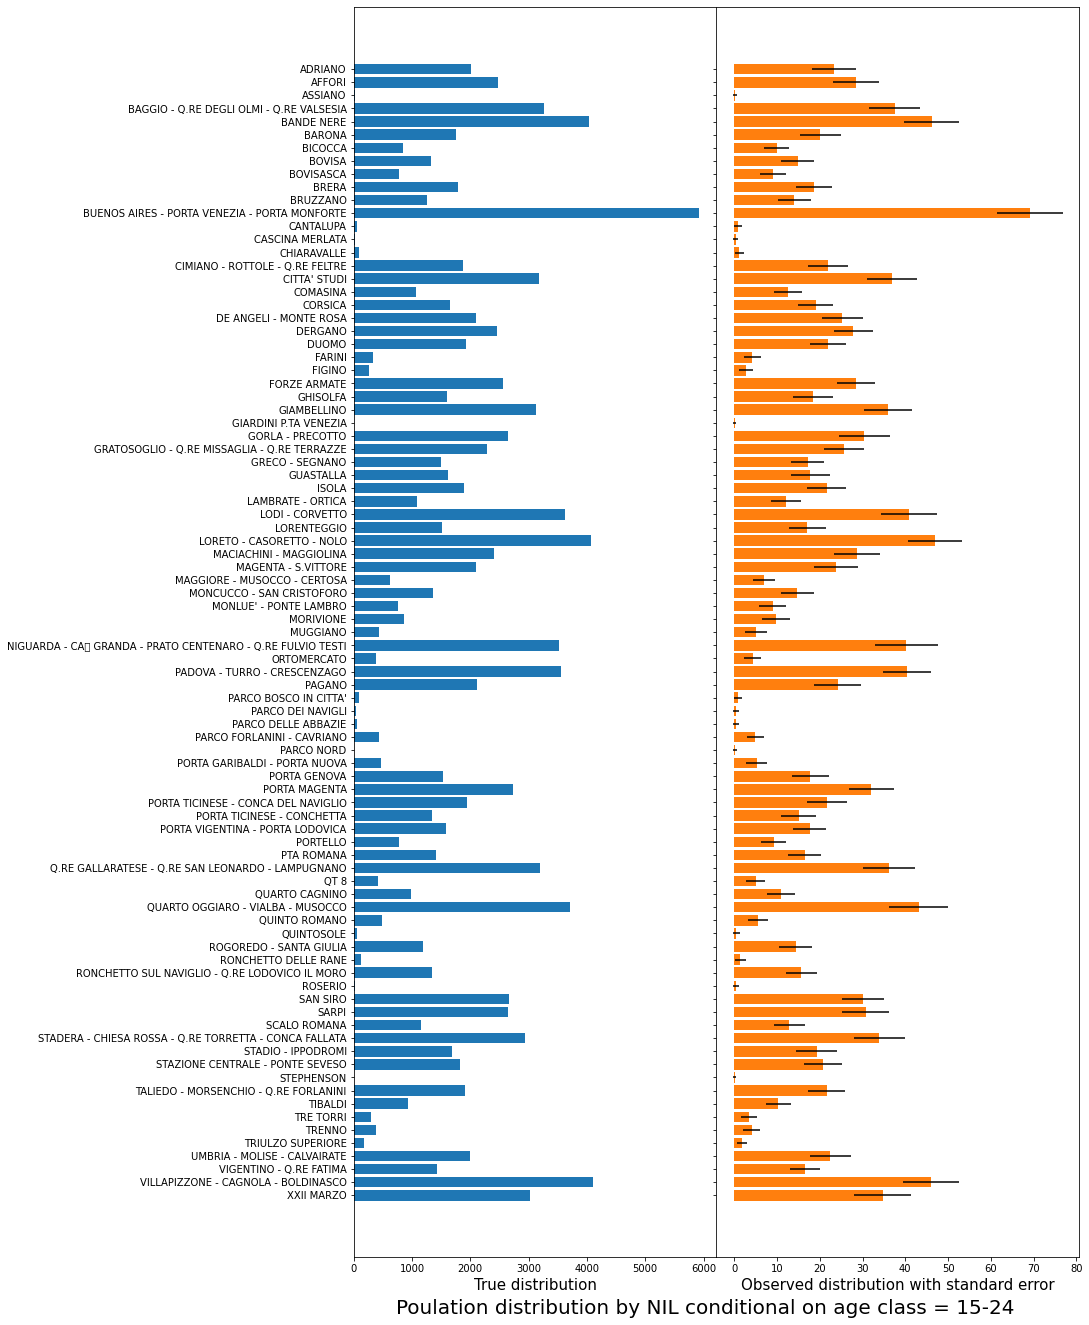
\includegraphics[scale = 0.45]{tex/pics/pop_by_nil_15.png}
    \caption{Comparison between the true population distribution by NIL (in blue) and the observed one (in orange) with standard error, conditional on agents being members of the 15-24 age class, averaged across 100 samples.}
    \label{pop_nil_15}
\end{figure}

\begin{figure}[H]
    \centering
    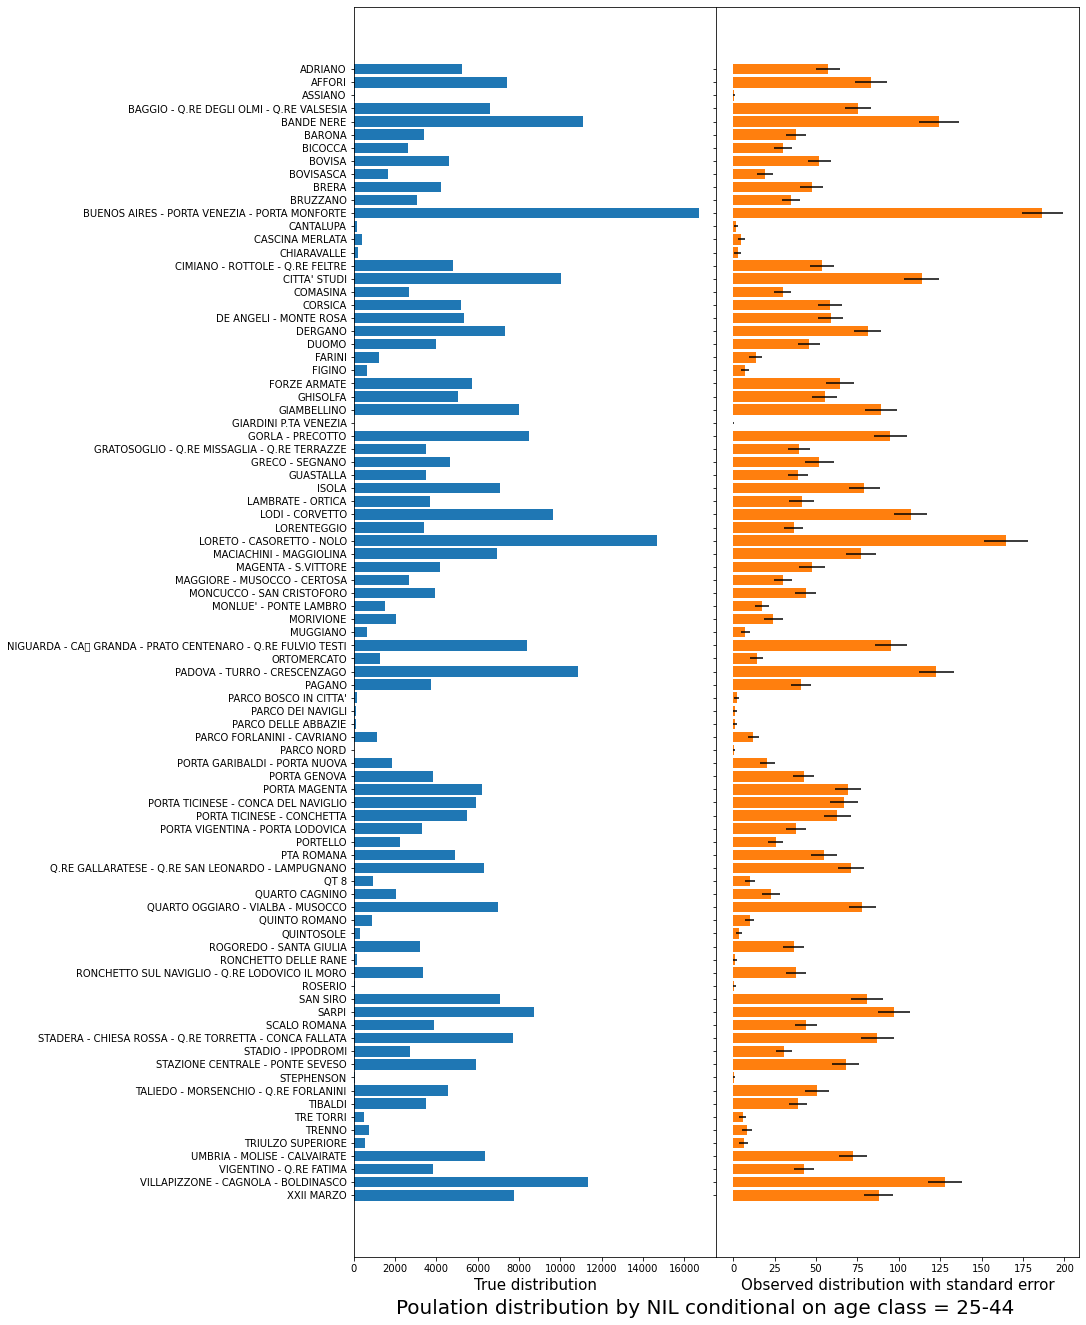
\includegraphics[scale = 0.45]{tex/pics/pop_by_nil_25.png}
    \caption{Comparison between the true population distribution by NIL (in blue) and the observed one (in orange) with standard error, conditional on agents being members of the 25-44 age class, averaged across 100 samples.}
    \label{pop_nil_25}
\end{figure}

\begin{figure}[H]
    \centering
    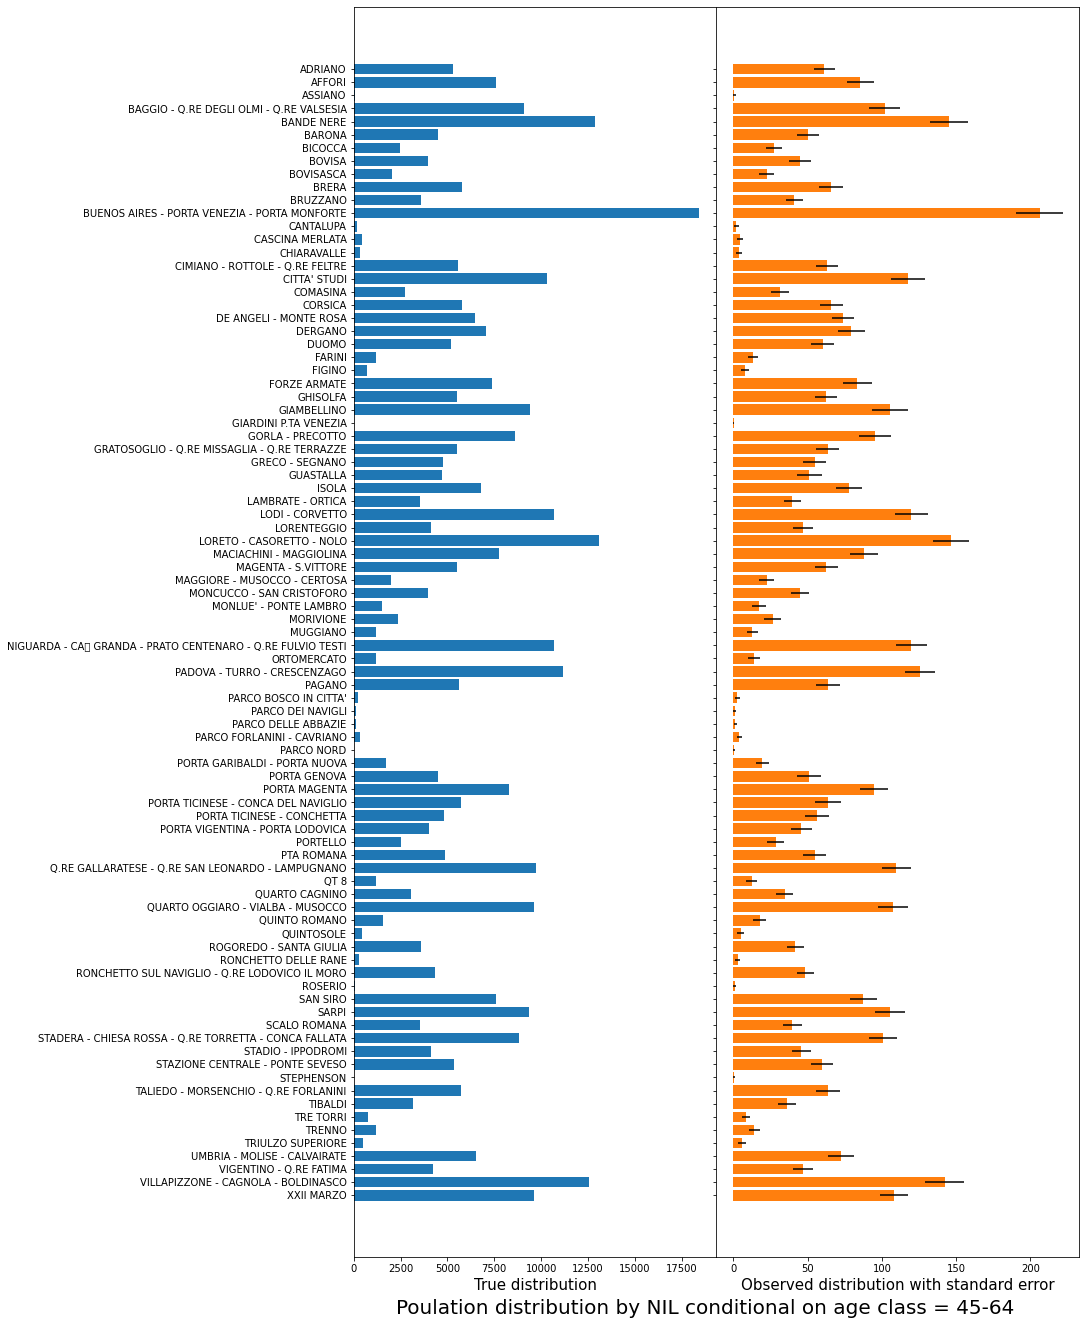
\includegraphics[scale = 0.45]{tex/pics/pop_by_nil_45.png}
    \caption{Comparison between the true population distribution by NIL (in blue) and the observed one (in orange) with standard error, conditional on agents being members of the 45-64 age class, averaged across 100 samples.}
    \label{pop_nil_45}
\end{figure}

\begin{figure}[H]
    \centering
    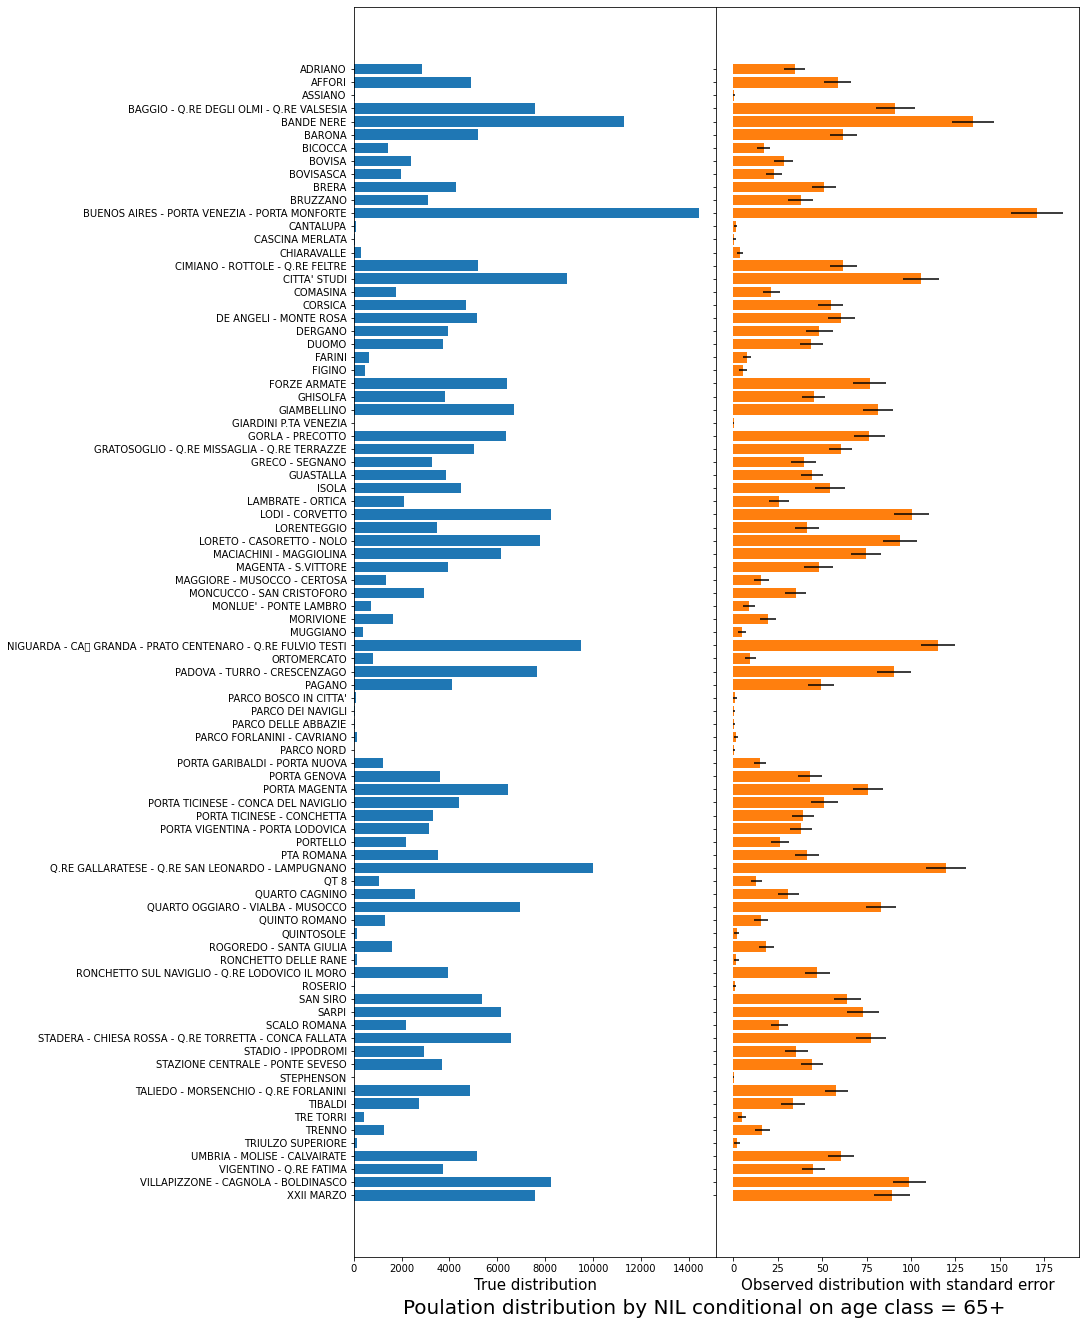
\includegraphics[scale = 0.45]{tex/pics/pop_by_nil_65.png}
    \caption{Comparison between the true population distribution by NIL (in blue) and the observed one (in orange) with standard error, conditional on agents being members of the 65+ age class, averaged across 100 samples.}
    \label{pop_nil_65}
\end{figure}





% \end{appendices}


\singlespacing
\printbibliography[heading=bibintoc,title={Bibliography}]

\end{document}
